%%%%%%%%%%%%%%%%%%%%%%%%%%%%%%%%%%%%%%%%%%%%%%%%%%%%%%%
% A template for Wiley article submissions.
% Developed by Overleaf. 
%
% Please note that whilst this template provides a 
% preview of the typeset manuscript for submission, it 
% will not necessarily be the final publication layout.
%
% Usage notes:
% The "blind" option will make anonymous all author, affiliation, correspondence and funding information.
% Use "num-refs" option for numerical citation and references style.
% Use "alpha-refs" option for author-year citation and references style.

\documentclass[num-refs]{wiley-article}
% \documentclass[blind,alpha-refs]{wiley-article}

% Add additional packages here if required
\usepackage{siunitx}
%\usepackage[colorinlistoftodos]{todonotes}
\usepackage{gensymb}

% Update article type if known
\papertype{Full Paper}
% Include section in journal if known, otherwise delete
% \paperfield{Journal Section}

\title{Molybdenum dichalcogenide cathodes for aluminium-ion batteries}

% List abbreviations here, if any. Please note that it is preferred that abbreviations be defined at the first instance they appear in the text, rather than creating an abbreviations list.
% \abbrevs{ABC, a black cat; DEF, doesn't ever fret; GHI, goes home immediately.}

% Include full author names and degrees, when required by the journal.
% Use the \authfn to add symbols for additional footnotes and present addresses, if any. Usually start with 1 for notes about author contributions; then continuing with 2 etc if any author has a different present address.
\author[1]{Shalini Divya}
\author[1]{James H. Johnston}
\author[2\authfn{1}]{Thomas Nann}

\contrib[\authfn{1}]{Corresponding author.}

% Include full affiliation details for all authors
\affil[1]{Victoria University of Wellington, School of Chemical and Physical Sciences, Wellington, New Zealand}
\affil[2]{The University of Newcastle, School of Mathematical and Physical Sciences, Callaghan, NSW 2308, Australia}

%\corraddress{Author One PhD, Department, Institution, City, State or Province, Postal Code, Country}
\corremail{thomas.nann@newcastle.edu.au}

%\presentadd[\authfn{2}]{Department, Institution, City, State or Province, Postal Code, Country}

\fundinginfo{No funding information available.}

% Include the name of the author that should appear in the running header
\runningauthor{Nann et al.}

\begin{document}

\maketitle

\begin{abstract}

Many successful battery electrodes are based on 2D-layered materials. We have studied aluminium-ion batteries using molybdenum dichalcogenides --- MoS$_2$, MoSe$_2$ and MoSSe as active cathode materials. The batteries exhibit clear discharge voltage plateaus in the ranges 1.6-1.4 V for MoS$_{2}$ and MoSe$_{2}$, and 0.6–0.5 V for MoSSe. While the MoSSe cathode exhibits a higher specific capacity over MoS$_2$ and MoSe$_2$ but the overall energy density is lower than MoSe$_2$ at a current density of 40 mA g$^-{^1}$, MoSe$_2$ proves to be a more stable cathode with a discharge specific capacity of 110 mAh g$^-{^1}$ with an average potential at $\approx 2.0 V$. Charge–discharge cycling at 100 mA g$^-{^1}$ demonstrates the stability of Al/MoSe$_2$ cell over 200 cycles with 90 \% coulombic efficiency. 

% Please include a maximum of seven keywords
%\keywords{aluminium-ion battery, molybdenum disulfide, molybdenum diselenide, ...}

\end{abstract}

\section{Introduction}
% You started to talk for 4 sentences about lithium. This is an aluminium paper!!!
 The aluminium-ion battery (AIB) anode redox couple Al$^3^+$/Al has a high theoretical, gravimetric capacity (2,980 Ah kg$^-^1$) when compared with Li$^+$/Li (3,862 Ah kg$^-^1$) and Na$^+$/Na (1,166 Ah kg$^-^1$). Futhermore, AIBs are low in cost, recyclable and the common ionic liquid electrolyte not inflammable. Although aluminium (Al) has a higher standard oxidation potential than lithium (Li), Al$^3^+$ cations result in a higher theoretical energy density compared to monovalent lithium (Li$^+$). Vanadium oxides such as V$_2$O$_5$ and VO$_2$ exhibited promising results but the intercalating Al$^3{^+}$ ions fixed themselves between the V$_2$O${_5}$ layers that made their diffusion very slow resulting in fewer charge/discharge cycles. Chiku \textit{et al} \cite{chiku_amorphous_2015} introduced an amorphous V$_2$O${_5}$/carbon composite where presence of highly electro-conductive Ketjenblack weakened the interaction between intercalating Al$^3^+$ ions and amorphous V$_2$O$_5$ layers, significantly improving the battery performance. Using X-ray photoelectron spectroscopy (XPS) analysis, the team found that the valency of vanadium changed while charging/discharging the cell. Two-dimensional vanadium carbide (MXenes)\cite{vahidmohammadi_two-dimensional_2017} were used based on a similar principle where Al$^3^+$ ions intercalated into the MXene layers and vanadium, V$^4^+$ reduced to V$^3{^+}$ during discharge and reversibly oxidised to V$^4^+$ during charge. Metal oxides such as MoO$_3$\cite{lahan_al3+_2019}, chevrel phase Mo$_6$S$_8$ \cite{geng_reversible_2015}, Ni$_3$S$_2$ \cite{wang_novel_2016}, MoS$_2$\cite{li_rechargeable_2018}, TiS$_2$\cite{geng_titanium_2017} and carbon-based materials have been tested as cathodes for AIBs. Materials with high surface area such as three-dimensional hierarchical CuS microspheres\cite{wang_high-performance_2017}, zeolite-template carbon\cite{stadie_zeolite-templated_2017} as an ordered microporous cathode, have shown better battery performance by providing shorter diffusion lengths thus making it easier for ions to intercalate or get absorbed onto the surface of the active material. 
Graphite has been a popular choice for cathodes in AIBs due to its layered structure. Various forms of graphite such as fluorinated graphite\cite{rani_fluorinated_2013}, Kish graphite flakes\cite{wang_kish_2017}, three-dimensional graphitic-foam\cite{lin_ultrafast_2015}, graphene mesh network\cite{chen_ultrafast_2017}, few-layer graphene aerogels\cite{qiao_defect-free_2019} and several other forms, have been tried as cathodes for AIBs, which showed discharge capacities ranging from 60-250 mAh g$^-{^1}$. The AlCl$_4^¯$ anions intercalate into the graphitic stacks and deintercalate during discharge. X-ray diffraction (XRD) and Raman spectroscopy studies have widely been used to establish the mechanism\cite{wang_advanced_2017}. Splitting of the graphite 002 peak 2 $\theta$ = 26.55, into two separate peaks indicated intercalation of AlCl$_4{^¯}$ anions resulting in highly strained graphene stacks.  During discharge, the pristine graphite peak reappears suggesting reversible intercalation /deintercalation of AlCl$_4^¯$ anions. Raman data revealed a doublet peak during charge, indicating vibration of carbon atoms in the interior graphite planes, which finally resulted in one single peak after the cell was fully charged indicating two stages of intercalation. While the cell discharged, pristine graphite spectra reappeared. XPS studies confirmed the reversible oxidation/reduction of carbon when AlCl$_4{^¯}$ anions intercalate/deintercalate respectively. While AlCl$_4{^-}$ ions act as the charge-carrying species for a few cathodes, MoS2 guy displayed intercalation of Al$^3{^+}$ ions when the cells discharged. Therefore, it can be said that a single mechanism for AIBs does not exist; it changes with every cathode material and its structure. 


\section{Results and Discussion}

Scheme 1 displays the crystal structure of MoX$_2$ where X = S or Se. The molecule has two vacant sites for intercalation - M1 and M2. M1 denotes the spaces in between the X-Mo-X bonds whereas M2, a larger site, is denoted by separation of two layers of MoX$_2$ with an inter-layer distance of 6.3\AA. The layers are held at this distance via van-der-Waals (vdW) forces. The M2 site presents an open network and various interstitial sites, which can easily accommodate the AlCl$_4^{-}$ anion, which are 5.28\AA\ in size as reported by Takahashi {\it et al}. An argument can be made about the kind of ion that participates in the intercalation process. Wang {\it et al.}\cite{li_rechargeable_2018} reported intercalation of Al$^{3+}$ cation during discharge. The triply charged Al$^3{^+}$ cation has to overcome the strong electrostatic force from the S$^2{^-}$ anion network to get in between MoS$_2$ layers; also, its participation is limited due to its tendency to form complexes when it intercalates. However, our preliminary tests showed  that participation of Al$^{3+}$ would rather \lq contract\rq\ the MoX$_2$ layers making AlCl$_4{^-}$ a probable choice.  Density Functional Theory (DFT) studies carried out by Pathak {\it et al.}, showed that AlCl$_4^-$ anions intercalated within the graphite system after distortion from its tetrahedral form due to vdW interlayer attraction forces between the host graphite layers. Here, we propose the intercalation of AlCl$_4^-$ anions into the M2 sites of MoX$_2$ during charging process. The electrochemical results, cyclic voltammetric scans, Raman spectroscopy and X-ray photoelectron spectroscopy results discussed later strongly support the reversible nature of the intercalation process.

\begin{figure}[t]
\centering
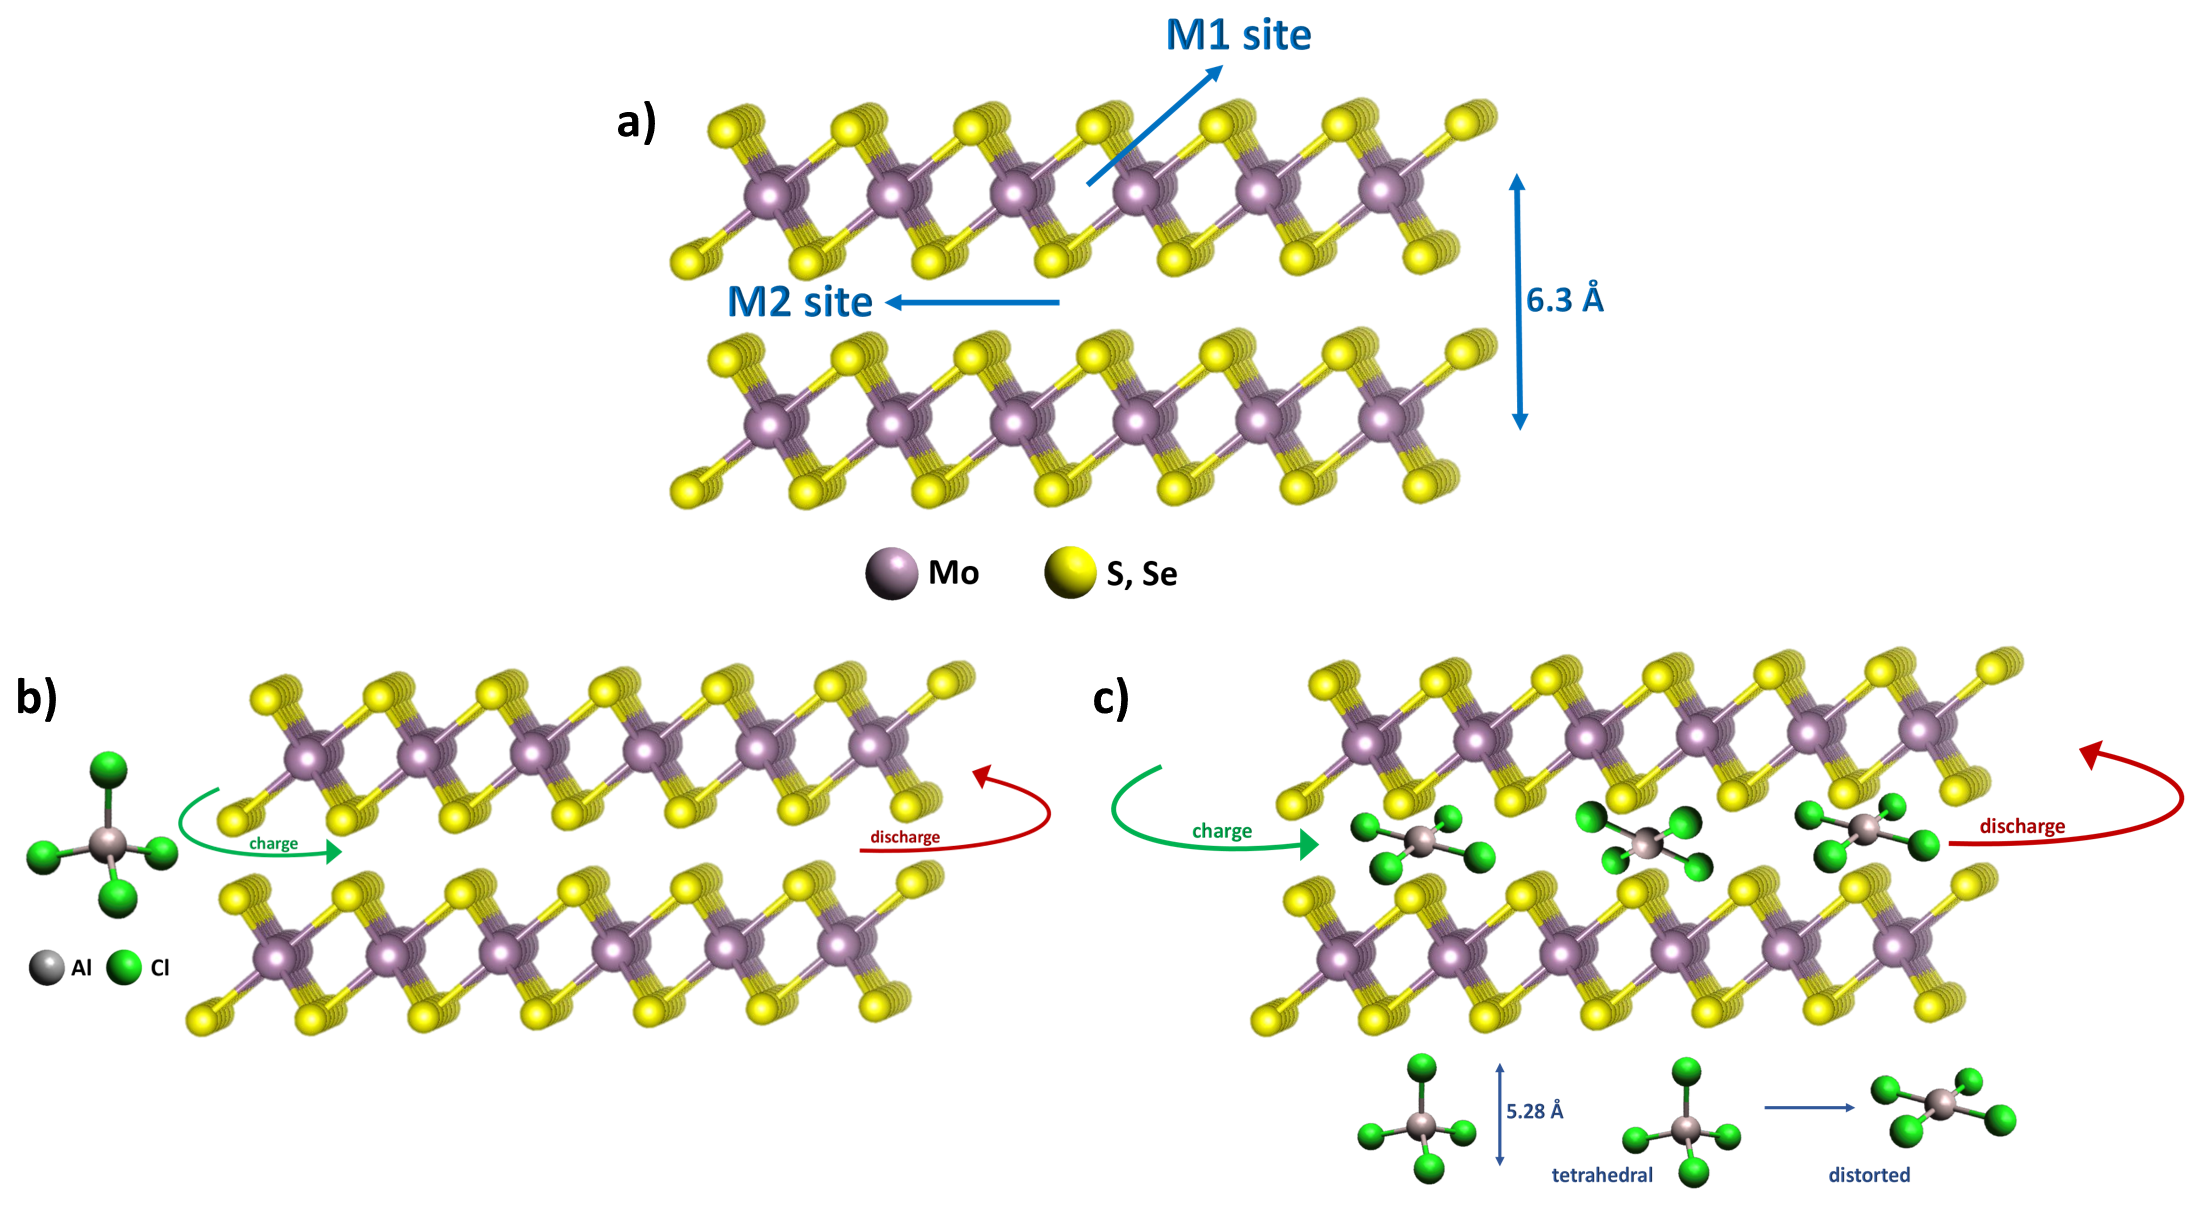
\includegraphics[width=\textwidth]{figures/S1}
\caption{Schematic representation of a) an MoX$_2$ crystal structure with possible intercalation sites at M1 and M2 b) intercalation at M1 site and c) intercalation at M2 site.}
\end{figure}

A modified two-electrode polyether ether ketone (PEEK) cell was used to make electrochemical measurements on aluminium-ion batteries (AIBs). Electrode preparations and cell configurations are described in the Methods section. After testing the molybdenum dichalcogenides for AIB cathodes, we found that in general, MoSe$_2$ was superior to MoS$_2$ and MoSSe, with higher and more stable capacities and distinct voltage plateaus. MoSSe was unstable with poor coulombic efficiency of $\sim$50\%. The cathode degraded rapidly after first few cycles and eventually became inactive after a few cycles. It seemed that sulphur substitution weakened the binding energy of Mo-Se allowing the bonds to break easily and thus resulting in rapid cathode degradation and hence, fading capacity. The presence of higher defects in the lattice structure of MoSSe (see XRD and Raman data) compared to MoS$_2$ and MoSe$_2$, contribute to its poor performance as a cathode material in AIBs.

\begin{figure}[h!]
\centering
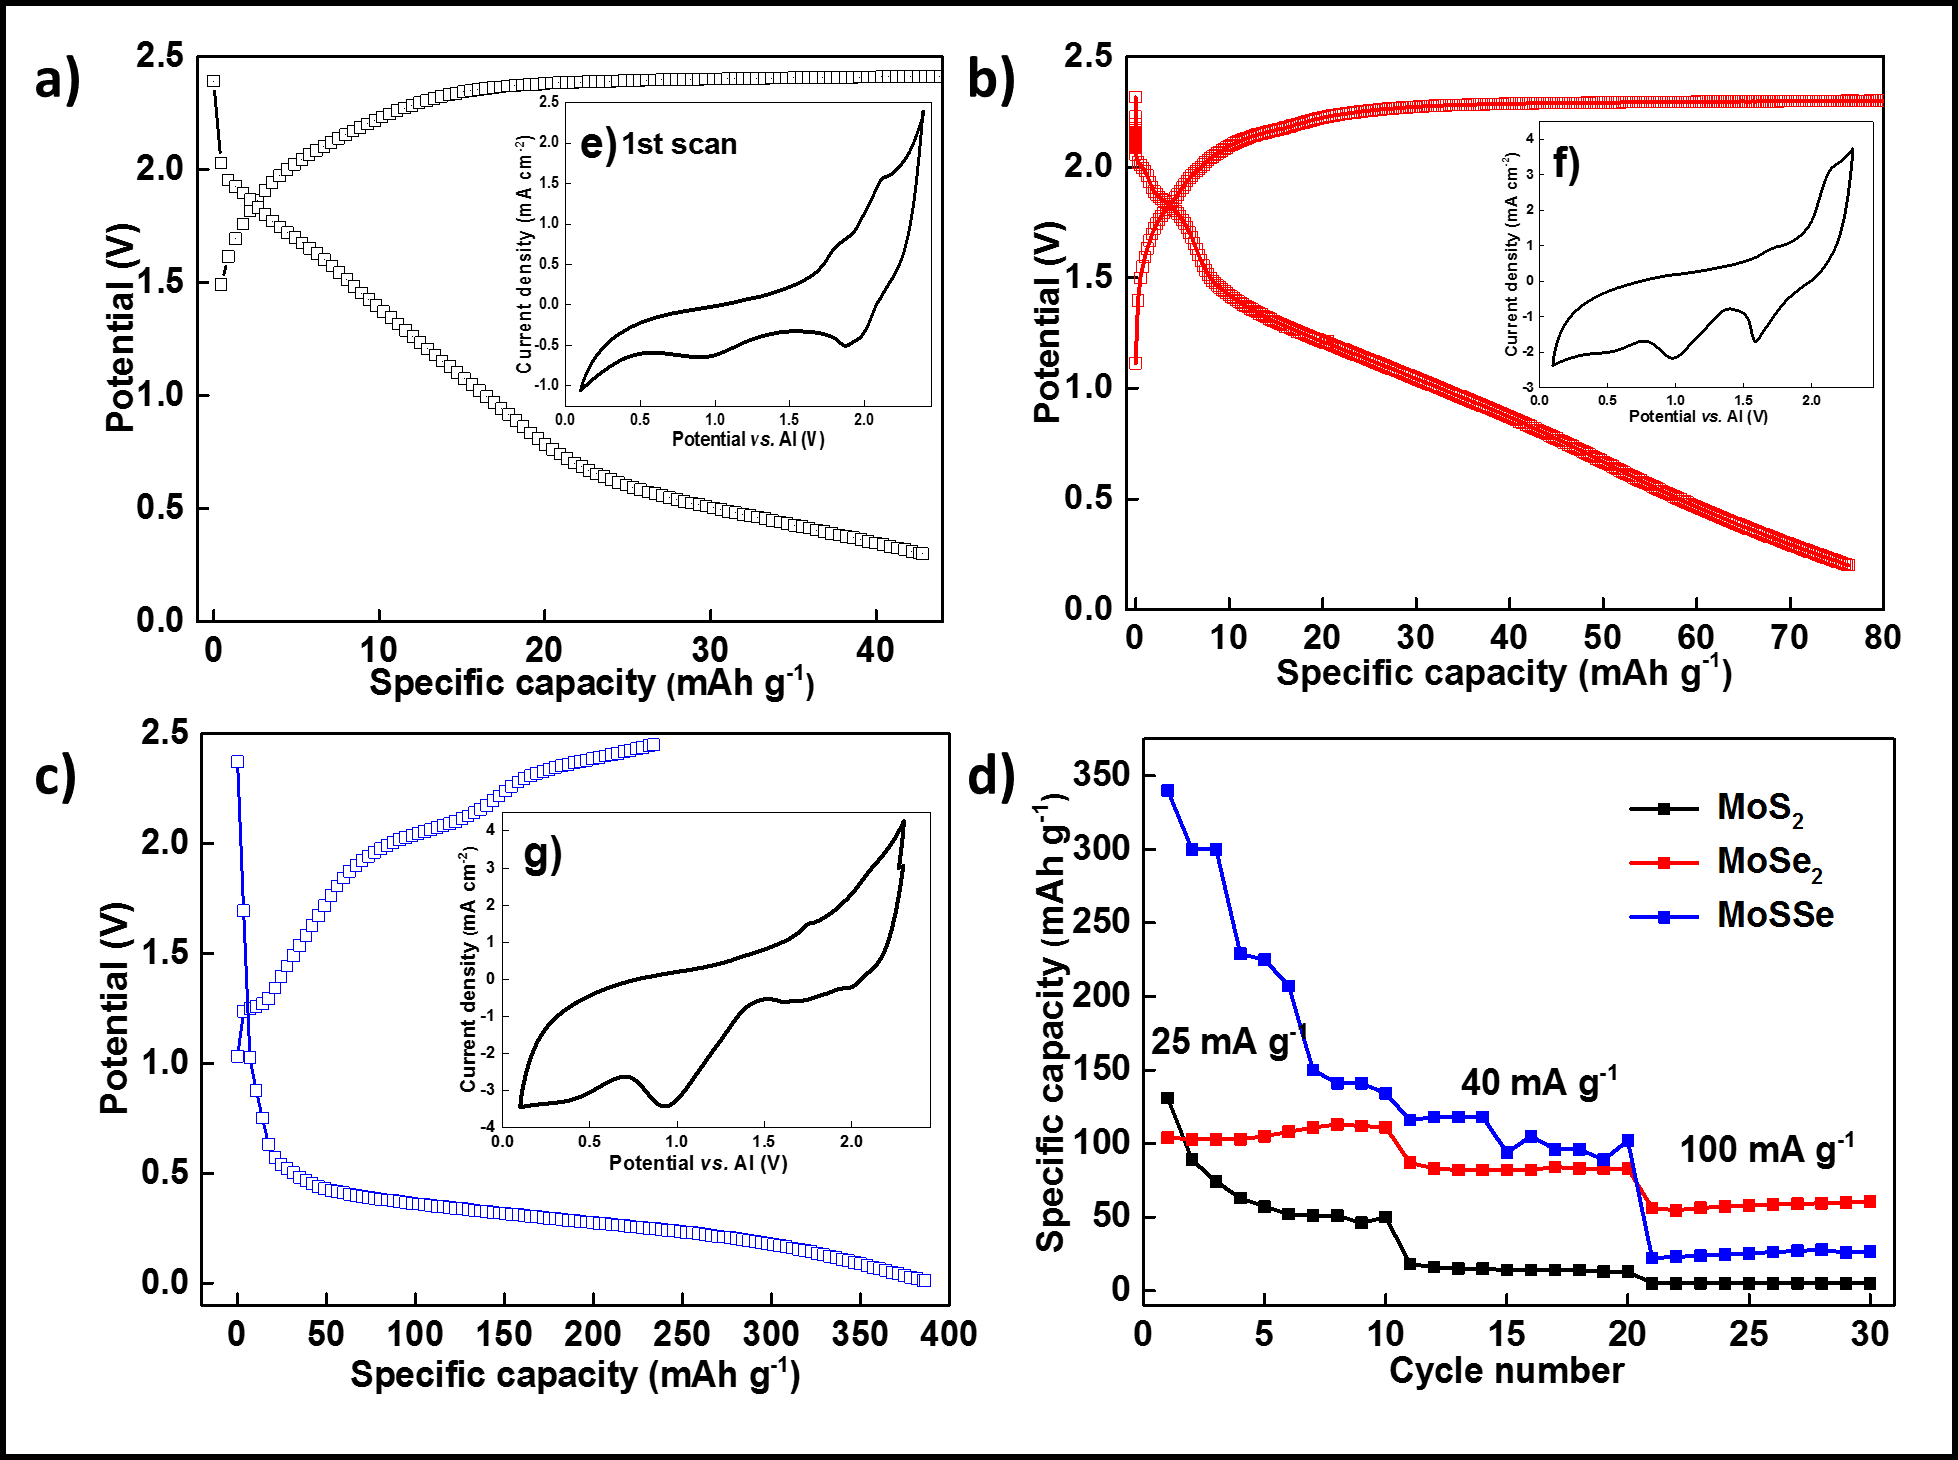
\includegraphics[width=\textwidth]{figures/fig1}
\caption{First charge/discharge curve at 40 mA g$^-^1$ for a) MoS$_2$, b) MoSe$_2$ and c) MoSSe.}
\end{figure}
% Figure 1 here


Figure 2 shows the charge/discharge curves (CDC) for MoS$_2$, MoSe$_2$and MoSSe. The discharge voltage was observed at 1.8 V and 0.6 V  for MoS$_2$, 1.9 V, 1.7 V  and 1.5 V for MoSe$_2$ and 0.5 V for MoSSe. For MoS$_2$, capacity recorded after first discharge was 43 mAh g$^{-1}$, which reduced to 40 mAh g$^{-1}$ and 31 mAh g$^{-1}$ in its second and third cycle respectively. We compared the cell's first CDC with its first cyclic voltammetry (CV) scan (Fig 1e-1g) and found a good resemblance between the discharging plateaus and reduction peak positions, and in between the charging plateau and oxidation peak positions. The two-step redox processes have good reversibility. Electrochemical performance of Al/MoSe$_2$ cell revealed some interesting results. With discharge plateaus at 1.9 V and 1.7 V, the first CV scan observed a reduction peak at 1.65 V and an irreversible peak at 1.0 V. The peak at 1.0 V disappeared after the first scan. This peak can be attributed to an irreversible phase transition that usually takes place in molybdenum dichalcogenides, in our case, MoSe$_2$, in its first cycle\cite{fan_hybrid_2017}. During this transition, a semi-conducting 2H phase converts to a more metallic 1T phase.  This transition works in favour of the cathode as it somehow increased the interlayer spacing of MoSe$_2$ (by reducing the vdW forces) and allowing more AlCl$_4^-$ ions to intercalate, thus leading to a higher capacity than MoS$_2$. From the CDC and CV scans, it is apparent that the redox processes are reversible even after 200 cycles (Fig SF1) at a higher current rate of 100 mAg$^{-1}$. Al/MoSSe cell observed three distinct plateaus during charge at 1.7 V, 2.0 V and 2.3 V in its first cycle with a low discharge plateau at 0.5 V. The presence of various charging potentials correspond to the oxidation processes that occur due to presence of both S and Se atoms. The first CV scan revealed an irreversible  reduction potential at 0.9 V (resembling MoSe$_2$), which disappeared after 1st cycle implying a similar irreversible phase transition. Only one reduction peak at 1.7 V was noted in the consecutive scans with decreased intensity after every cycle. However, no plateau was observed in the CDC for MoSSe at that potential. Performance of the three electrodes was observed at different current rates (25, 40 and 100 mA g$^-^1$). MoSe$_2$, recorded the most stable capacities at all potentials compared to MoS$_2$ (recording the lowest capacity of 11 at 100 mA/g) and MoSSe (recording a significant drop ion capacity after a few cycles at all current rates). 
\begin{figure}[h!]
\centering
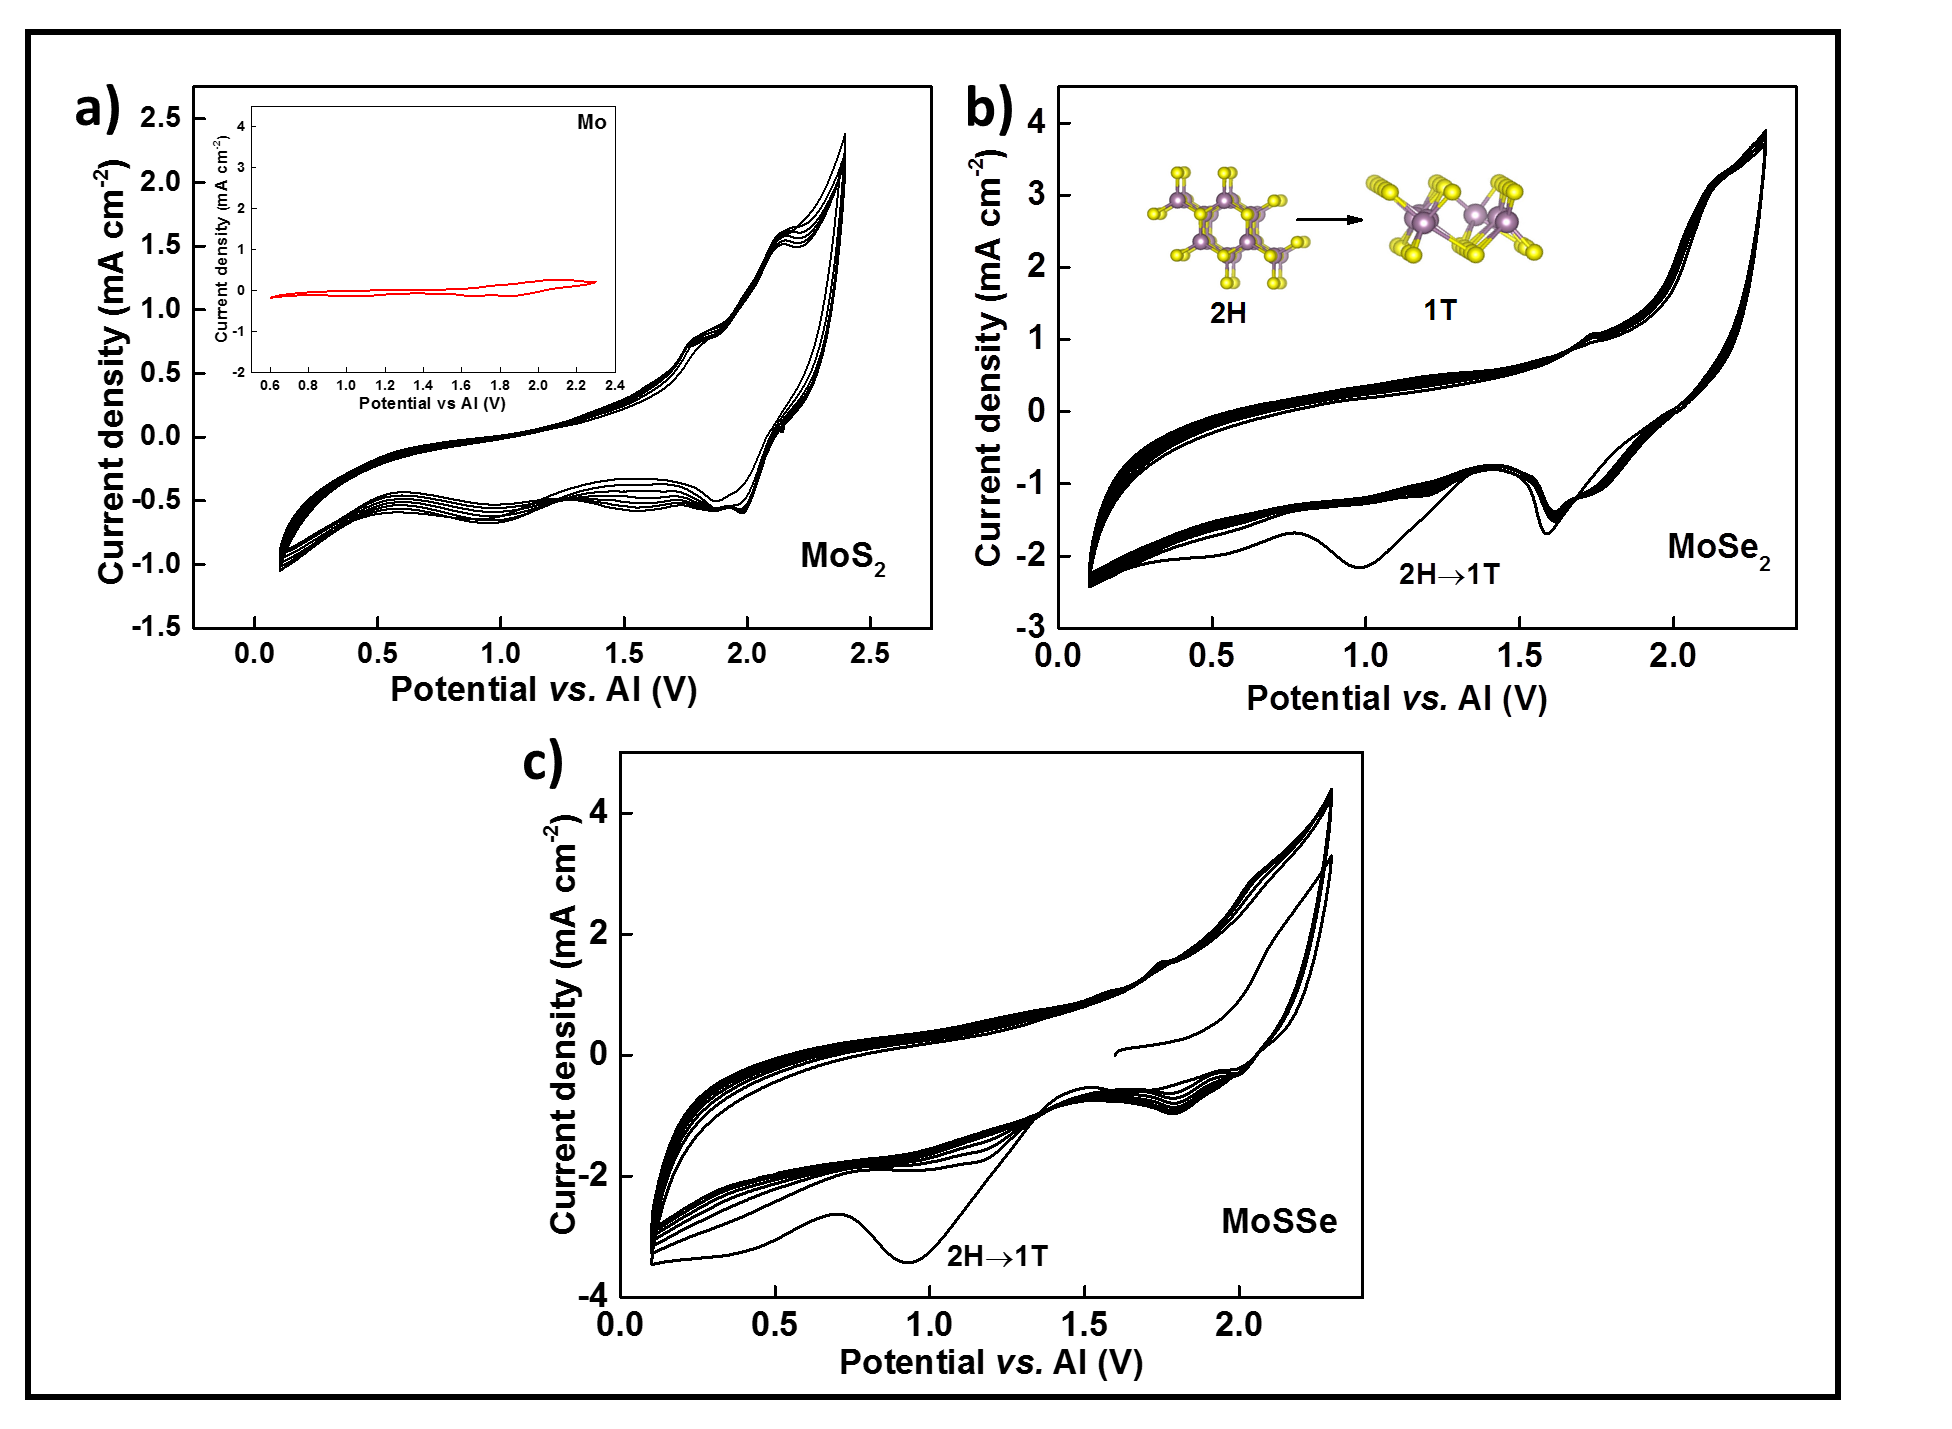
\includegraphics[width=\textwidth]{figures/fig2}
\caption{Cyclic voltammograms of a) MoS$_2$, b) MoSe$_2$ and c) MoSSe at a scan rate of 10 mV s$^-^1$..}
\end{figure}
% Figure 2 here

Both MoS$_2$ and MoSe$_2$ have similar interlayer distance (6.5 \AA) but MoSe$_2$ recorded a higher capacity and a more stable cycle life than MoS$_2$. To account for this behaviour, we observed the CV scans of all electrodes. Different charge storage mechanisms can lead to different CV curves. Firstly, we noted that MoSe$_2$ (Fig 3b) and MoSSe (Fig 3c) had a higher CV area than MoS$_2$ (Fig 3a). In addition, the phase transition for MoSe$_2$ and MoSSe (2H$\rightarrow$1T) is prominent in their first scan at 0.9 V - 1.0 V. No such transitions were observed for MoS$_2$. Charge storage in MoS$_2$ seems to be primarily based on redox processes (reversible intercalation of AlCl$_4^-$ ions) : reversible oxidation and reduction peaks observed at 1.8 and 2.1 V, and 2.0 V respectively. A rectangular CV suggests towards an electrocapacitive mechanism. MoSe$_2$ indicated towards both a reversibe redox process (intercalation/deintercalation) and an electric double-layer charge storage because of its rectangular looking CV curve from 0.1 v to 1.5 V. The surface-induced charge storage might have resulted in an additional capacity.  CV scan of MoSSe, which lacked evidence for any reversible redox process due to absence of clear oxidation/reduction peaks, derives its capacitance mainly from a surface phenomena. CV curve from Mo foil (Fig 3a inlet)proved that capacitance in all the cells came solely from the active material and not the current collector.
\begin{figure}[h!]
\centering
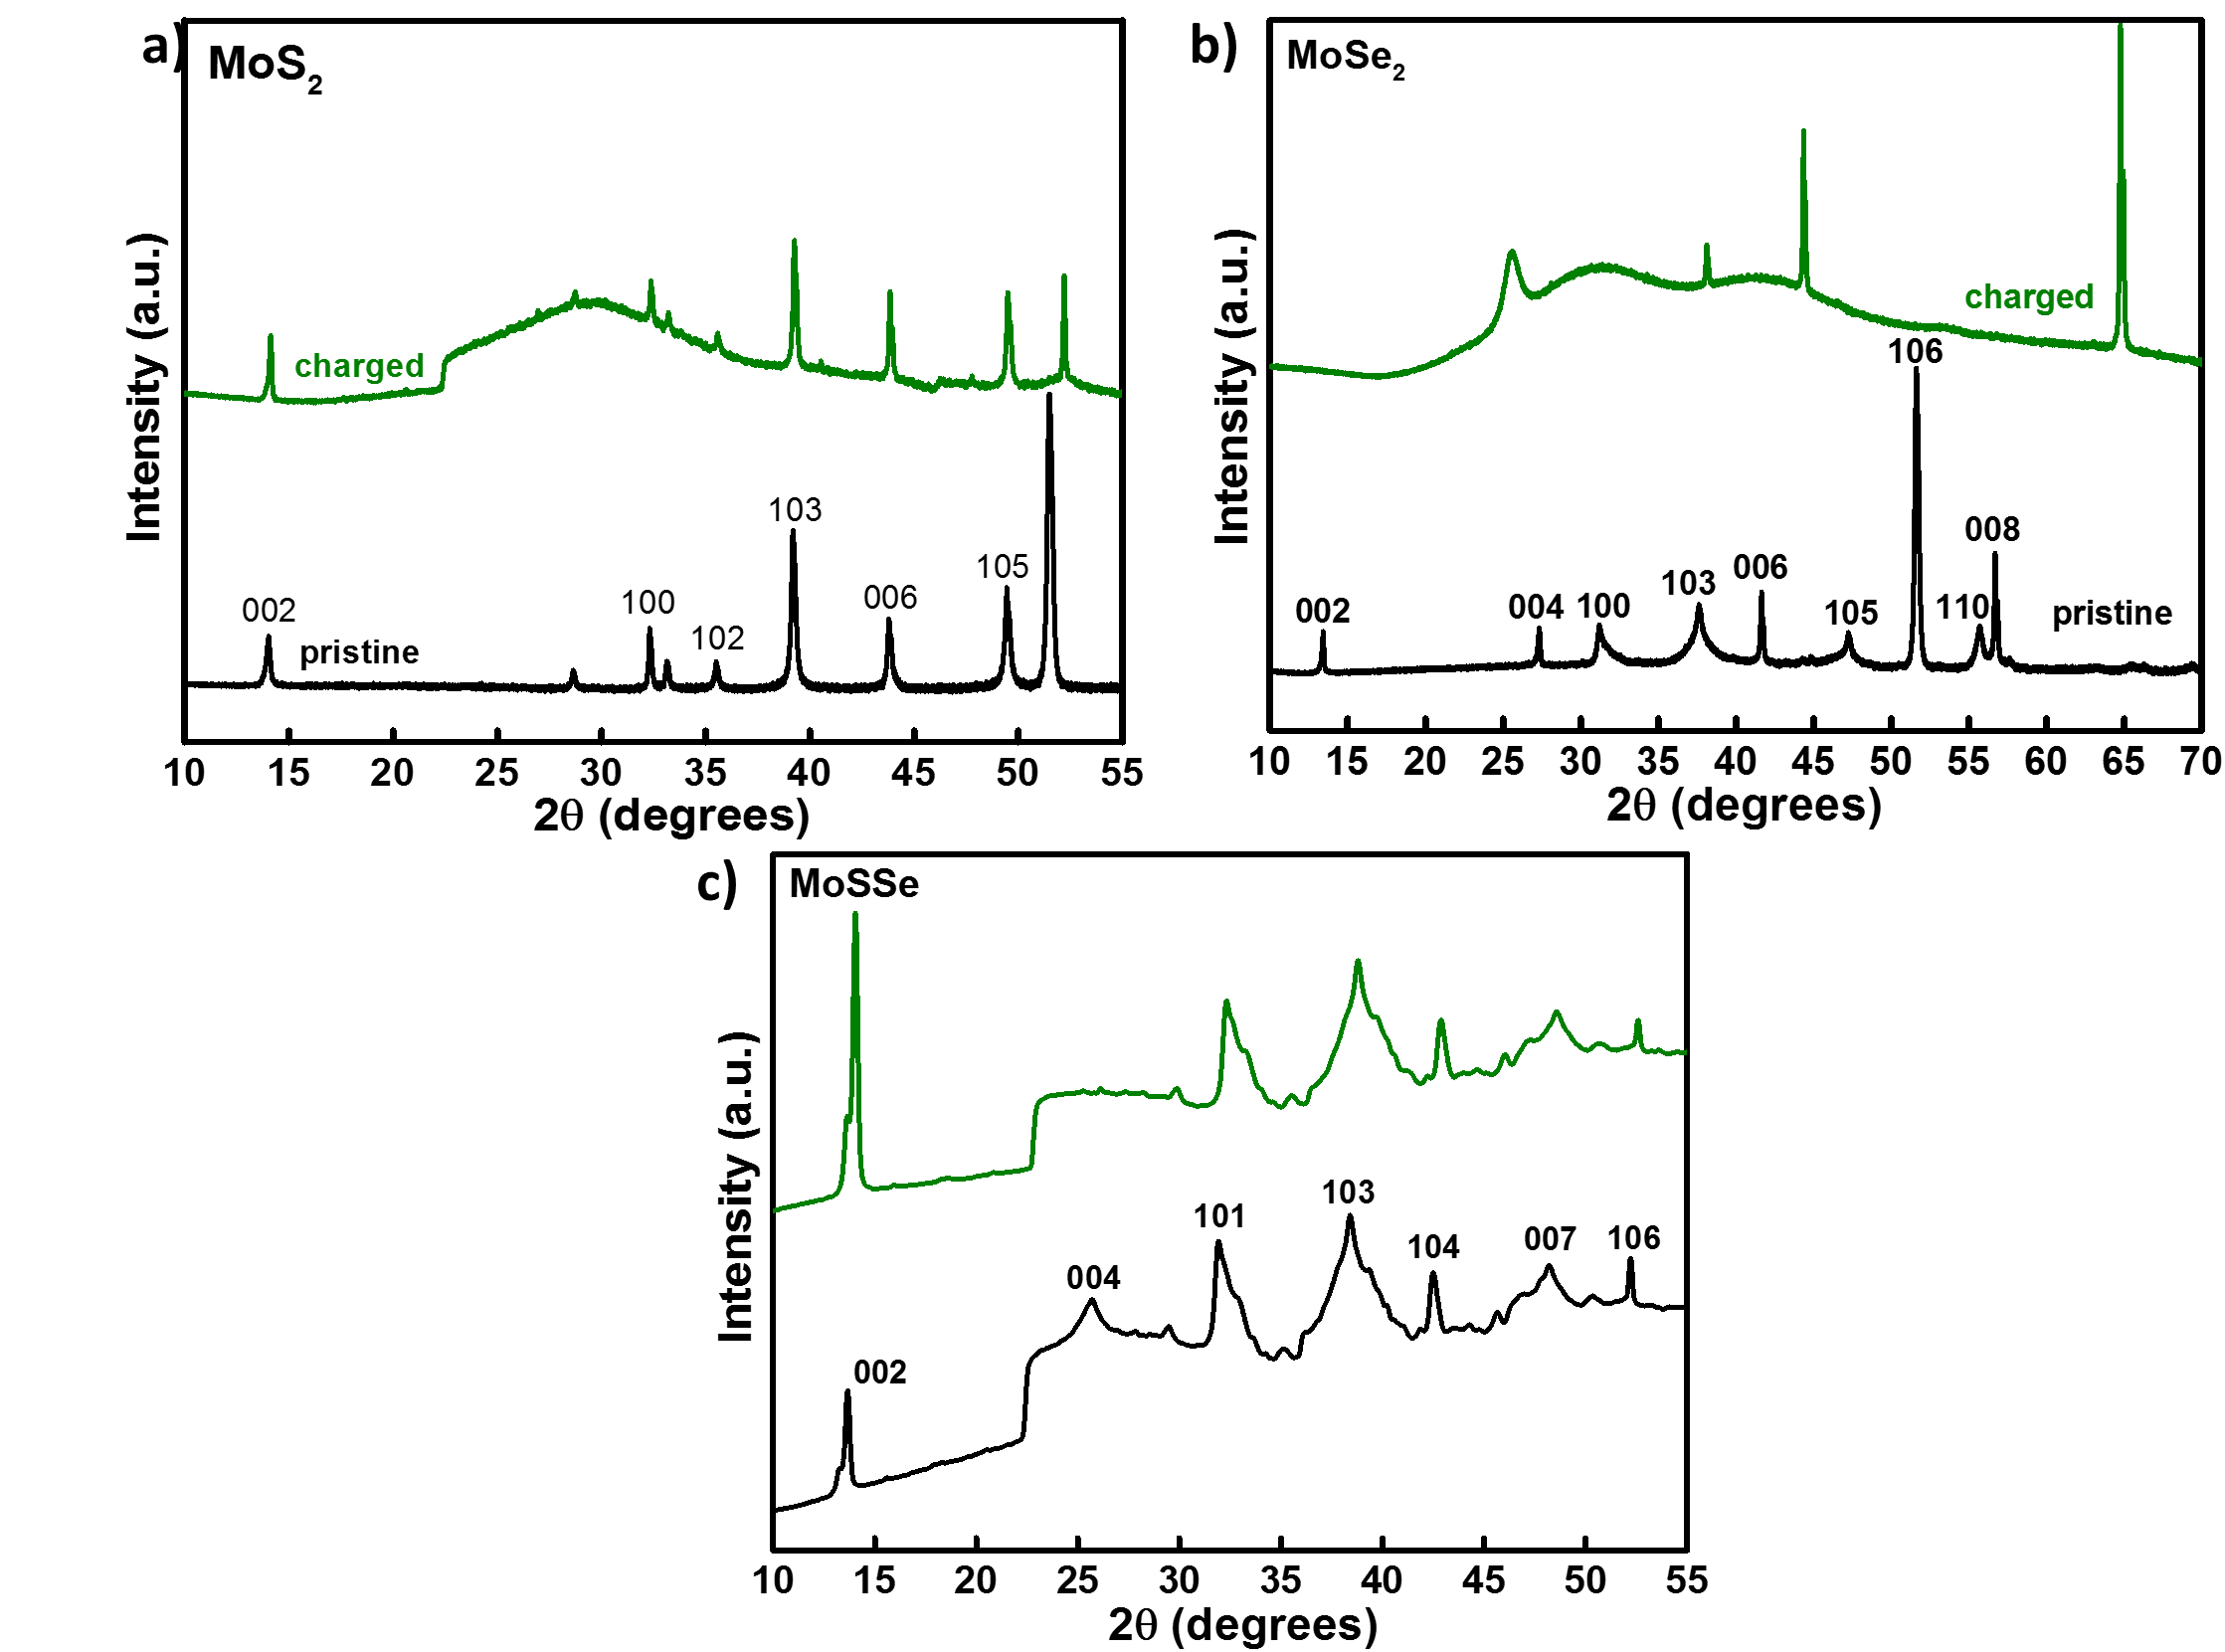
\includegraphics[width=\textwidth]{figures/fig3}
\caption{X-ray diffraction spectra of pristine (black) and charged (green) a) MoS$_2$, b) MoSe$_2$ and c) MoSSe.}
\end{figure}
%Figure 3 here....

Figure 4 displays the X-ray diffraction measurements of MoS$_2$, MoSe$_2$ and MoSSe electrodes. XRD spectra for MoS$_2$ (Fig 4a) compares the pristine (verified by JCPDS No. 17-0744) and charged electrode. It was seen that the 002 plane shifted from 14.21\degree\  to 14.02\degree suggesting a very small increase in the inter-layer distance of the layered molecule. The amorphous nature of the charged electrode was expected as the cell was cycled 20 times which might have changed the lattice structure a little. Most of the peaks retained their positions suggesting no significant loss in its crystal lattice. MoSe$_2$, on teh other hand, displayed significantly shifted peaks after charge. The diffraction peak at 2$\theta$ values of 13.4\degree\ (002) disappeared after charging, whereas the peaks at  27.28\degree\ (004), 41.64\degree\ (006) and 51.59\degree\ (106) shifted to 25.58\degree\ , 38.08\degree\  and 44.38\degree\ respectively. A decrease in theta values of 004 and 006 planes (along the c-axis of the molecule) indicate an increase in the inter-layer spacing of the molecule. These observations strongly suggest intercalation of distorted AlCl$_4^-$ ions during charge. Phase transformation that converts 2H to 1T contributes to the change in lattice structure of MoSe$_2$.The presence of amorphous peaks (at 33\degree\ and 42\degree\ ) suggest the same. MoSSe, however, does not have a well-defined crystal structure to begin with, as is evident from the XRD spectra of the pristine electrode (Fig 3c, in black). These defects might have formed during sulphur substitution in the Mo-Se bond making the Mo-Se bond weaker. Not only does this substitution impact the crystal structure of the molecule, but also results in degradation of the cathode when bigger AlCl$_4^-$ ions start to interact with them.The shift of 002 plane and disappearance of the 004 plane is a result of intercalation of AlCl$_4^-$ ions in the first few cycles and phase transformation.Overall, the molecule retains its lattice after 20 cycles, confirming the surface-based interaction of the anions which does not alter the crystal structure unlike MoSe$_2$. 

\begin{figure}[h!]
\centering
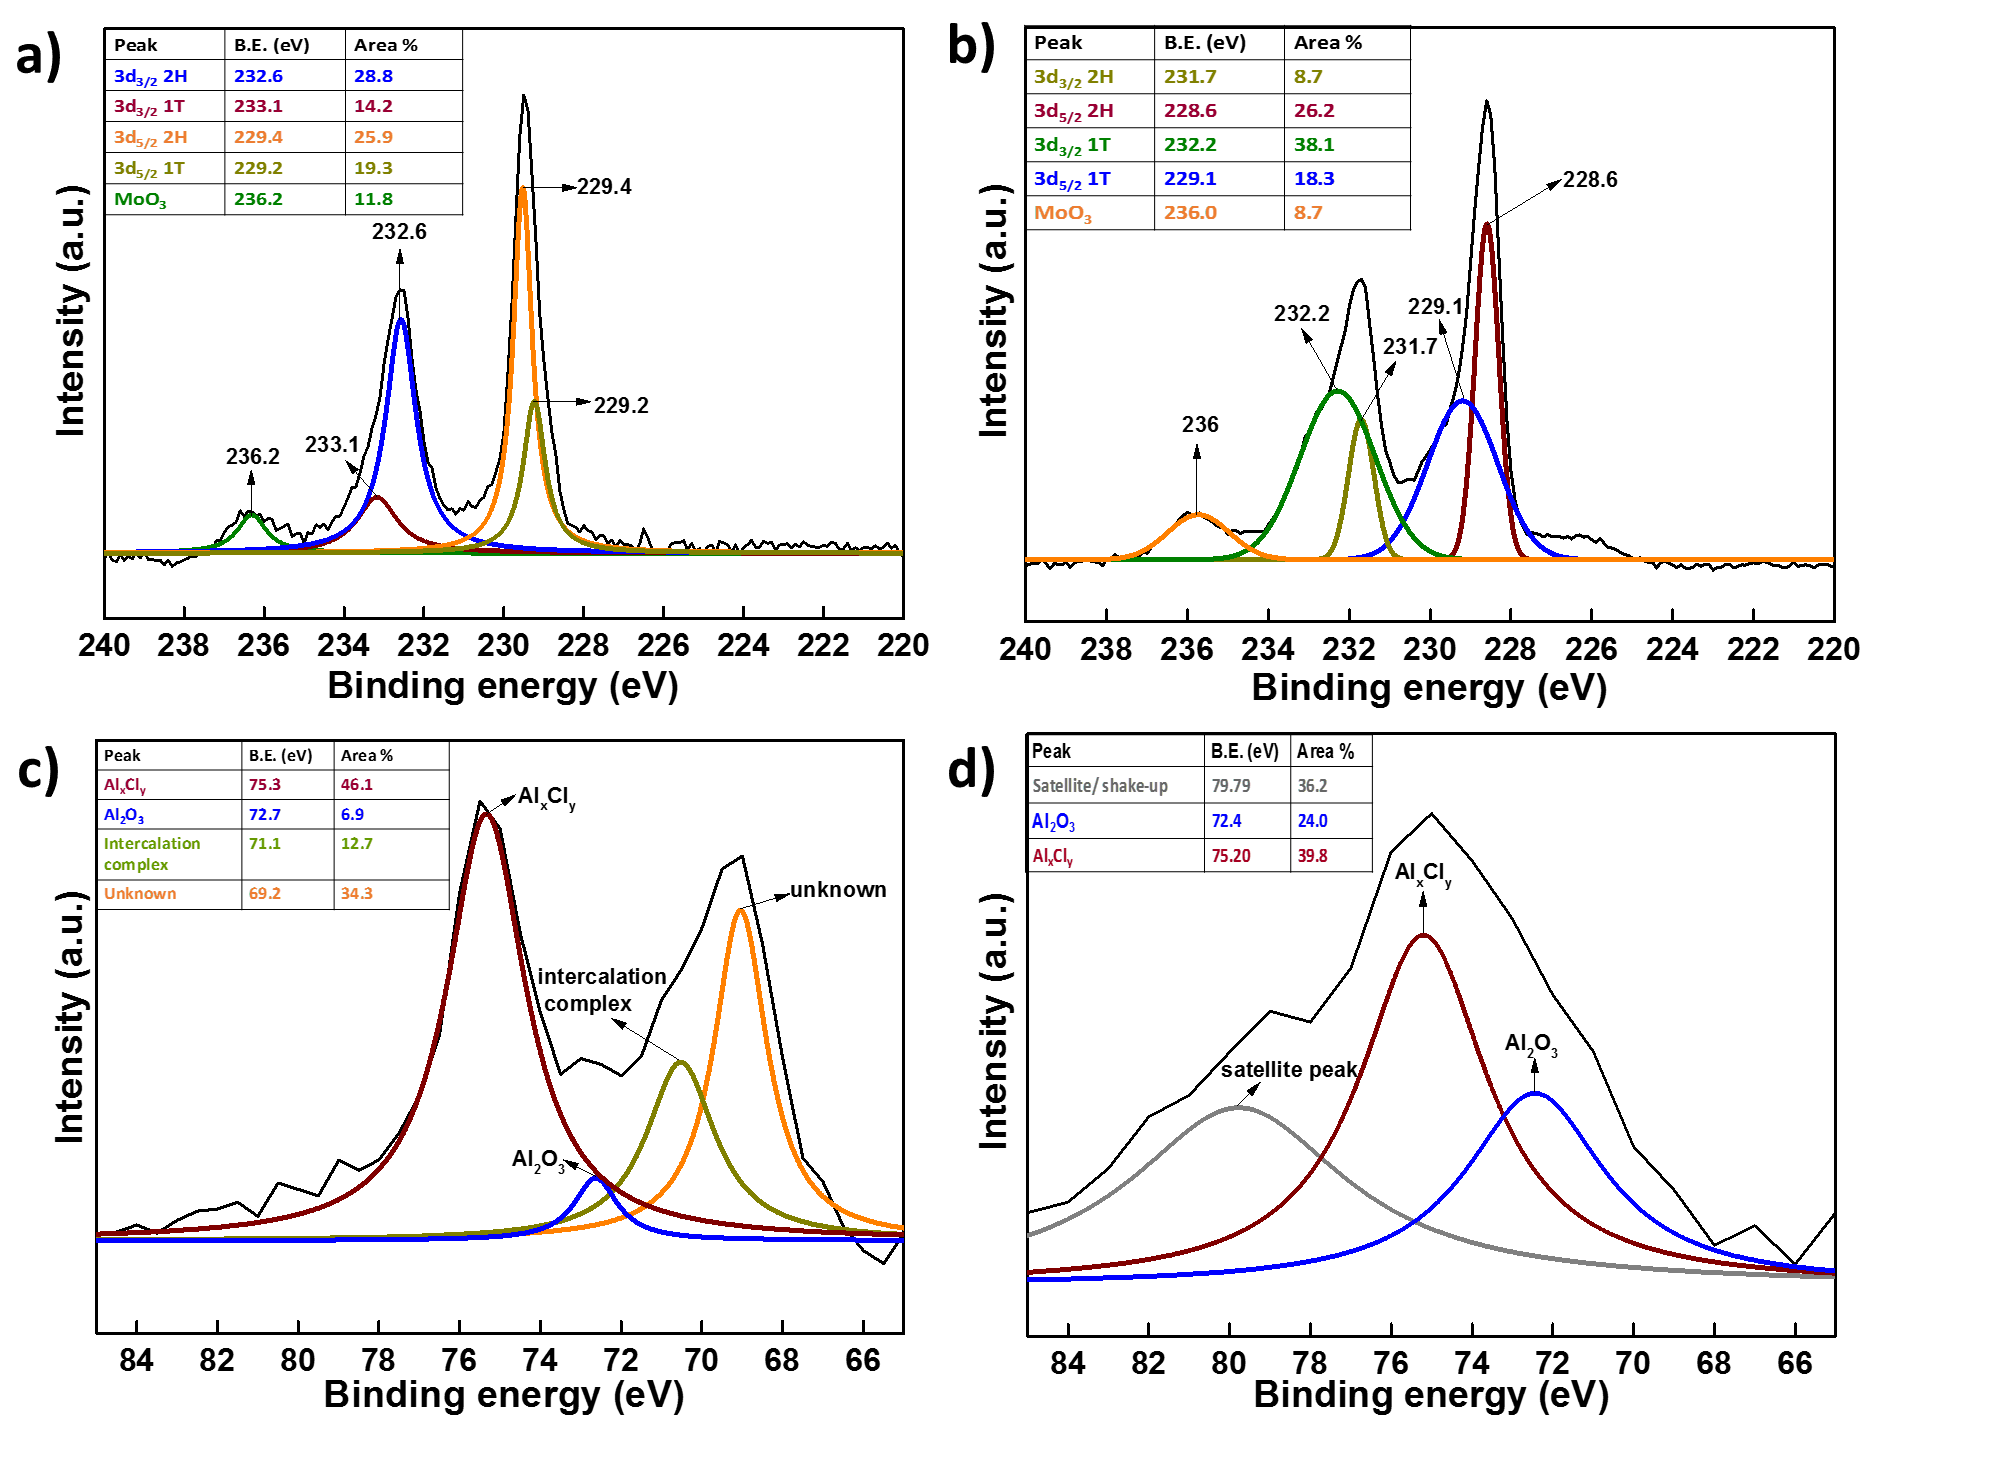
\includegraphics[width=\textwidth]{figures/fig4}
\caption{XPS spectra of Mo 3d orbital in a charged a) MoSe$_2$ and b) MoSSe electrode and Al 2p orbital in a charged c) MoSe$_2$ and d) MoSSe electrode.}
\end{figure}
% Figure 4 here.

To confirm the intercalation of AlCl$_4^-$ in MoSe$_2$, X-ray photoelectron spectroscopy (XPS) was used, which is a useful tool in distinguishing various oxidation states and helps in identifying different polymorphs (2H and 1T) especially in transition metal dichalcogenides . Detailed narrow spectrum scan (Figure 4) displays the binding energy of Mo (3d$_5_/_2$ and 3d$_3_/_2$) and Al 2p peaks for charged MoSe$_2$ and MoSSe electrodes. For pristine MoSe$_2$ electrodes, the binding energy of Mo 3d observed two peaks at 229.1 eV and 232.2 eV corresponding to 3d$_5_/_2$ and 3d$_3_/_2$ and Se 3d included a doublet at 55.4 eV and 54.6 eV corresponding to Se 3d$_3_/_2$ and 3d$_5_/_2$ respectively (Fig). Since peak splitting in an XPS spectrum indicates a phase change or a change in oxidation state, the spectra for the charged electrodes looked significantly different. The peak for Mo 3d split into three doublets indicating Mo$^4^+$ (from pristine MoSe$_2$), Mo$^5^+$ (formed after cell was charged) and Mo$^6^+$ (from formation of MoO$_3$). The pristine electrode of MoSSe (SF) already contained Mo in more than one oxidation states or suggested presence of both polymorphs (2H and 1T) . After charge, the peak areas increased for Mo 3d peak at 231.7 eV and 228.6 eV corresponding to 3d$_5_/_2$ and 3d$_3_/_2$ respectively (Fig 5b) . Increase in the area of 1T polymorph can be confirmed from the first CV scan. In addition, the doublet for Se 3d was replaced by one broad peak, which can be deconvoluted into four peaks further confirming the presence of more than one oxidation state and a new polymorph. A new peak at ~236 eV in Mo 3d spectra for MoS$_2$, MoSe$_2$ and MoSSe electrodes (Fig , Fig 5a and 5b) corresponds to Mo$^6^+$ species from MoO$_3$ after exposure of the electrode in air. XPS probing for Al 2p showed presence of Al in all charged electrodes of MoS$_2$ (Fig S), MoSe$_2$ (Fig 5c) and MoSSe (Fig 5d). MoSe$_2$ electrode displayed binding energies of Al 2p at 77 eV and 76eV corresponding to chlorides (Al$_x$Cl$_y$) and Al$_2$O$_3$ respectively. After AlCl$_4^-$ ions intercalated into MoSe$_2$ layers, a new peak at 69 eV was detected. we attribute this peak to a new complex that indicates a new environment for Al. Further analysis is required to confirm this species. Charged MoSSe electrode displayed broad peaks at 74.5 eV and 76 eV (Fig 5d) indicating presence of a higher amount of Al$_2$O$_3$ and chloroaluminate ions respectively. High atomic ratio of Al$_x$Cl$_y$ might come from electrolyte residue on the cathode's surface. The XPS data helps in confirming that intercalation of AlCl$_4_-$ ions definitely take place in case of MoSe$_2$, leading to a complex that reversibly forms during charge/discharge. 

\begin{figure}[h!]
\centering
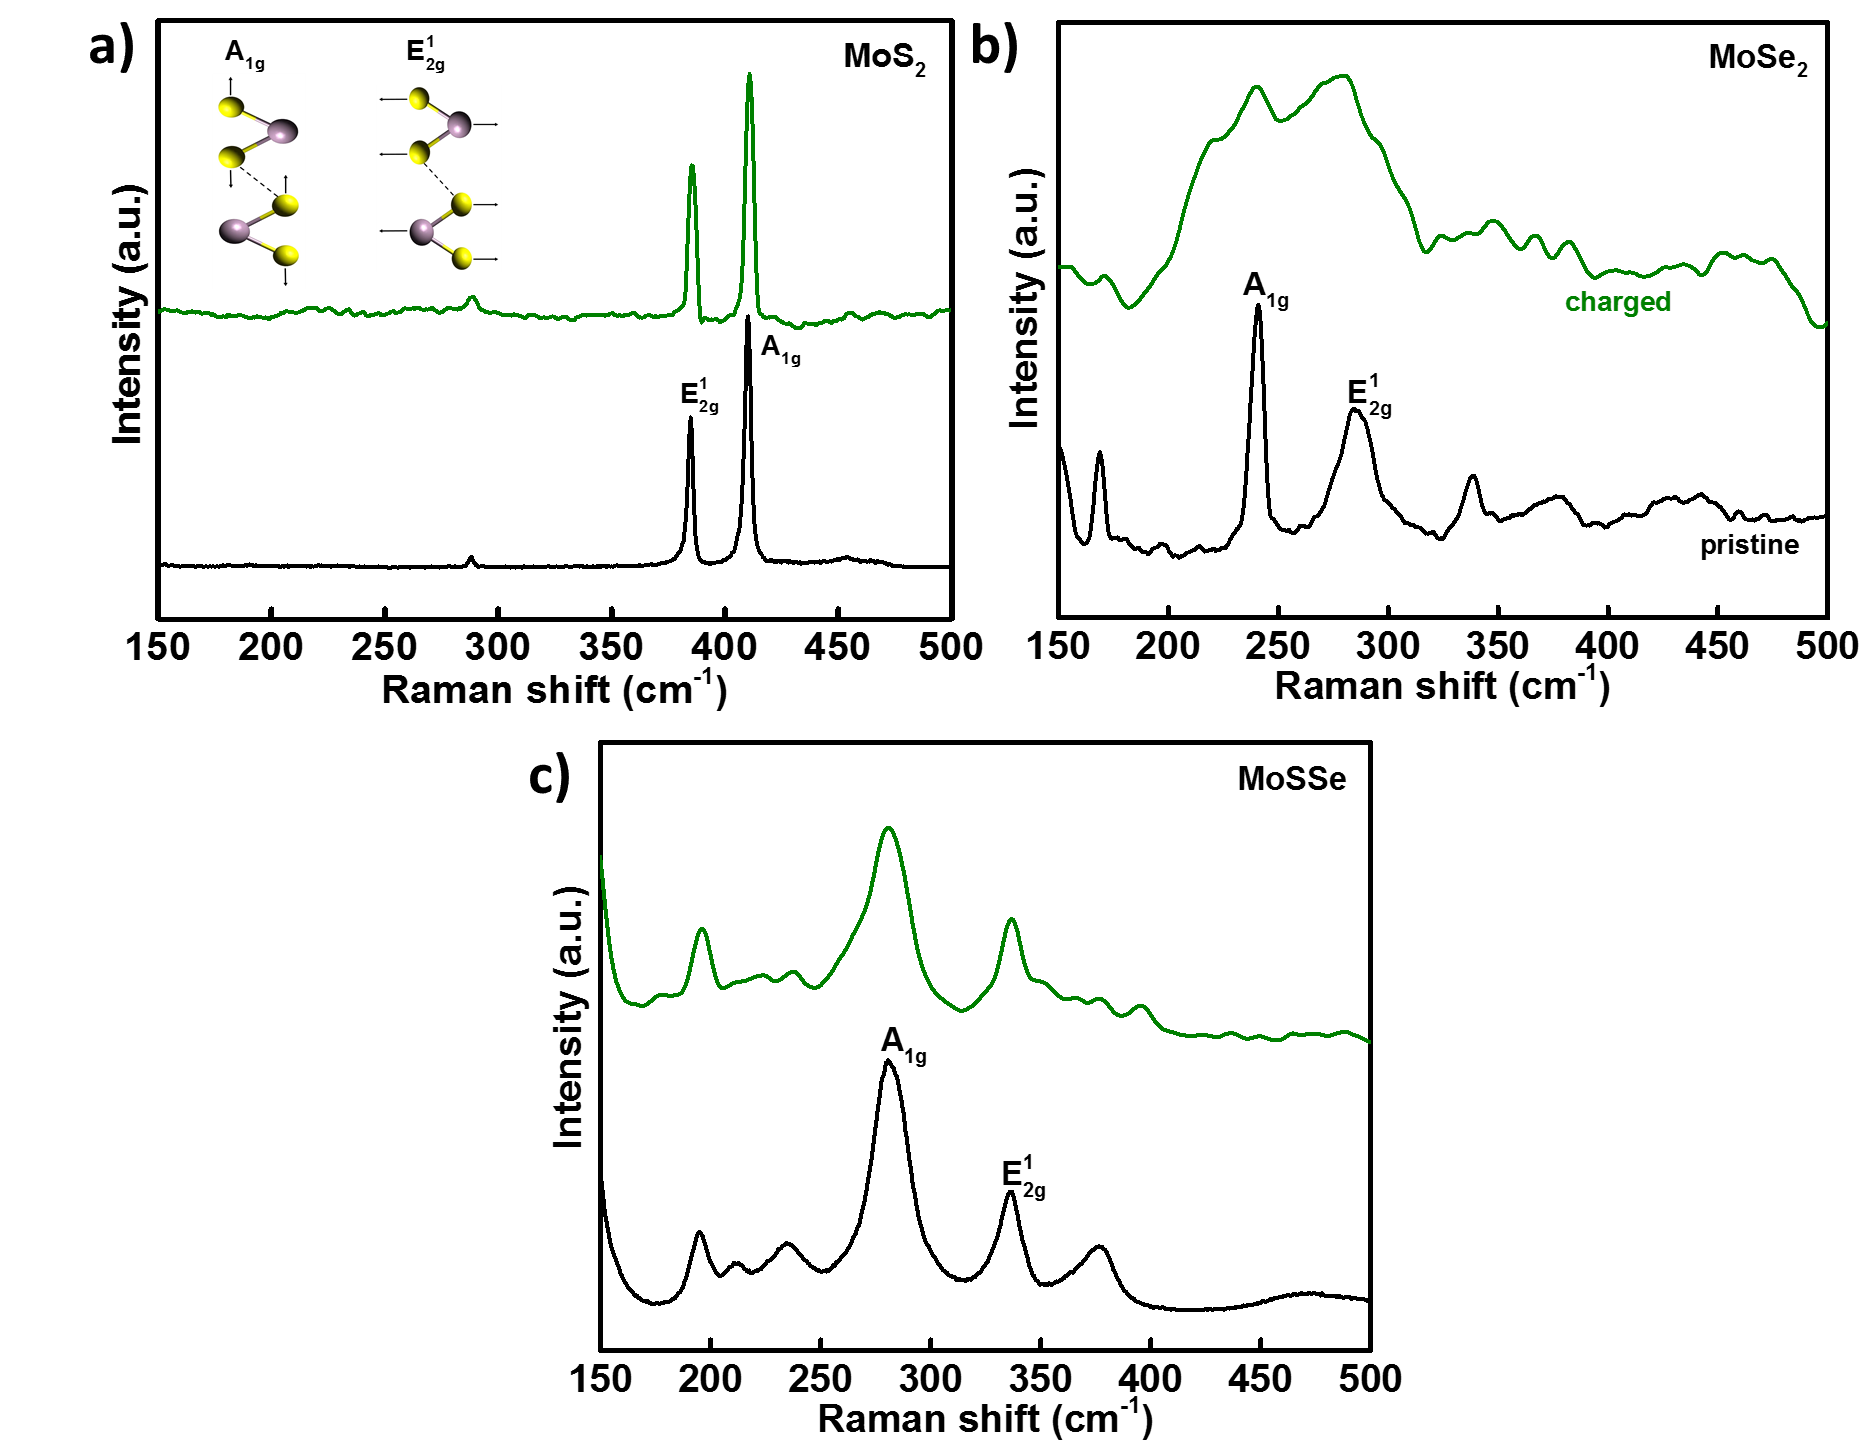
\includegraphics[width=\textwidth]{figures/fig5}
\caption{Raman spectra of pristine (black) and charged (green) a) MoS$_2$, b) MoSe$_2$ and c) MoSSe electrode .}
\end{figure}
% Figure 6 here


In addition we compared the Raman spectra of pristine and charged electrodes of MoS$_2$, MoSe$_2$ and MoSSe to detect any shift in the vibrational modes of the molecule. Two peaks corresponding to E$^1_2_g$ and A$^1_g$ vibrational modes for MoS$_2$ (Fig 6a) are prominent at 384.6 cm$^{-1}$ and 410.2 cm$^{-1}$ respectively. A$^1_g$ indicates an out-of-plane symmetric displacement of S atoms, whereas E$^_2_g$ suggests an in-layer displacement. Also, a separation between the two modes indicates a multilayer structure, which is observed for all three materials. No significant peak shift or peak broadening was observed for the charged MoS$_2$ electrode when compared to its pristine electrode. Raman spectra of MoSe$_2$ (Fig 6b) displayed broadening of A$_1_g$ peak at 240.6 cm$^{-1}$, which shifted to 239.3 cm$^{-1}$ after intercalation of AlCl$_4^-$ ions and E$^1_2_g$ peak at 284.5 cm$^{-1}$ shifted to 279.2 cm. These shifts and peak broadening after charge indicate an increase in lattice defect sites and a possible phase transition. Absence of a phase conversion might be the reason why MoS$_2$ does not record any peak broadening unlike MoSe$_2$ and MoSSe. This confirms our previous results where we observed phase transition for MoSe$_2$ and MoSSe but not MoS$_2$. Fig 6c showed the vibrational modes of MoSSe with A1g peak at 281.2 cm$^{-1}$ and E12g at 336.4 cm$^{-1}$. A$_1_g$ peak in the pristine MoSSe electrode broadened after intercalation of AlCl$_4^-$ ions but the change was not as significant as MoSe$_2$. Raman results confirm our XRD results suggesting MoSe$_2$ underwent a significant structural change after intercalation of AlCl$_4^-$ ions. 


\section{Conclusions}
In summary, MoSe$_2$ exhibited a higher capacity and cyclic stability than MoS$_2$ and MoSSe, as the cathode material for AIBs. The CV and XPS results indicated an irreversible phase transition from 2H to a more metallic 1T phase. We found from our XRD, XPS and Raman results that AlCl$_4^-$ seemed to intercalate reversibly into MoSe$_2$ (with a possible formation of a complex), whereas there was little evidence for intercalation into other molybdenum dichalcogenides.  A DFT analysis is crucial to determine the nature of this complex. This proposed intercalation along with a little electro-capacitive behaviour, resulted in an increased performance of MoSe$_2$ electrodes. The battery had a high average voltage of ∼2.0 V, and it delivers a specific capacity of about 80 mAh g$^−{^1}$ with nearly 95$\%$ coulombic efficiency at a current density of 40 mA g$^{−^1}$ making MoSe$_2$ a a promising cathode material for rechargeable AIB applications.


\section{Experimental Section}
\subsection{Cathode preparation}
Slurry was prepared by mixing MoX$_2$ (85$\%$ by wt.), 9$\%$ binder (PVDF, MTI Corporation) and 6$\%$ Super-P conductive carbon (99+$\%$ metals basis, Alfa Aesar) in N-methyl pyrrolidone NMP (anhydrous, 99.5$\%$, Sigma-Aldrich). It was ‘doctor-bladed’ on molybdenum foil (thickness 0.1 mm, MTI Corporation) and dried in a vacuum oven at 120°C for 12 hours to adhere the slurry on the conductive substrate and evaporate the solvent. Specific loading of hBN was 12 mg cm$^-{^2}$. 
\subsection{Electrolyte preparation}
Anhydrous AlCl$_3$ (Sigma-Aldrich) and EMImCl (97$\%$, Sigma-Aldrich) were mixed in a molar ratio of 1.3:1, at room temperature. EMImCl was baked in vacuum for 24 hours at 100°C to remove residual moisture. Small aliquots of AlCl$_3$ was added to EMImCl after every few minutes. The ionic liquid was stirred for 2-3 hours until a clear brown liquid was obtained. Since the electrolyte is hygroscopic in nature, it was prepared in a N$_2$-filled glove box with <0.1 ppm H$_2$O/O$_2$. 
\subsection{Cell assembly}
PEEK (polyether ether ketone) cells were used for electrochemical measurements. Molybdenum rods were used as current collectors. MoX$_2$ coated on molybdenum foil was used as the cathode and placed at bottom of the cell. Two glass microfibers (Grade GF/F, Whatman) were used as separators. 80µl of the electrolyte was used to wet the separator. Aluminium foil (thickness 0.1 mm, 99$\%$, GoodFellow) used as an anode and placed on top of the separator. The cell was then sealed and wrapped with a paraffin film to avoid any air or moisture contact. It was assembled in a N$_2$-filled glove box. Since this was a two-electrode setup, aluminium foil was used as both counter and reference electrode. The cell was taken out of the glove box and electrochemical measurements were performed. 
\section*{Supporting Information}
Supporting  Information  is  available  from  the  Wiley  Online  Library  or  from the author.
\\The cells recorded a higher charging capacity in their first cycles when compared to their discharging capacities. Since intercalation of AlCl$_4^-$ takes places during charging, the irreversible capacity can be attributed to the dissociation of Al$_2$Cl$_7^-$ ions at the electrode surface, or formation of an SEI layer may also render a few side reactions that take place on the electrode-electrolyte interface at such high potentials. 
\begin{figure}[h!]
\centering
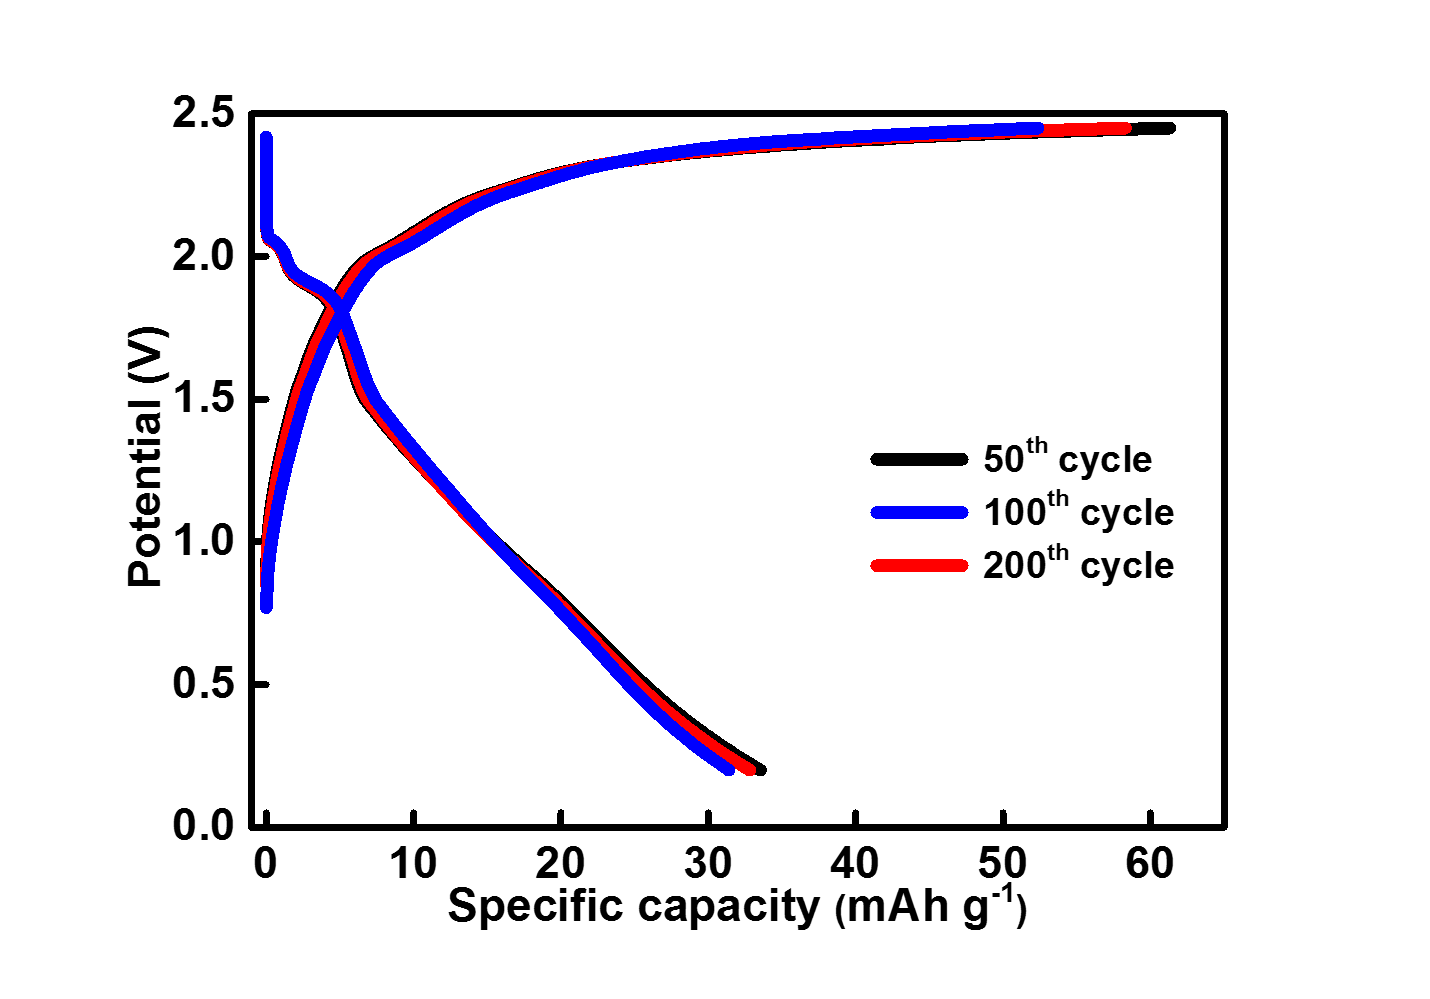
\includegraphics[width=\textwidth]{SF/SF1}
\caption{Rate- stability test of MoSe$_2$ at 100 mA g$^-^1$. \\Since MoSe$_2$ performed better than MoS$_2$ and MoSSe, we performed long-term cycle tests to test the cycle life. Cell capacity was retained after 200 cycles at a higher current rate of 100 mA g$^-^1$.}
\end{figure}


\begin{figure}[h!]
\centering
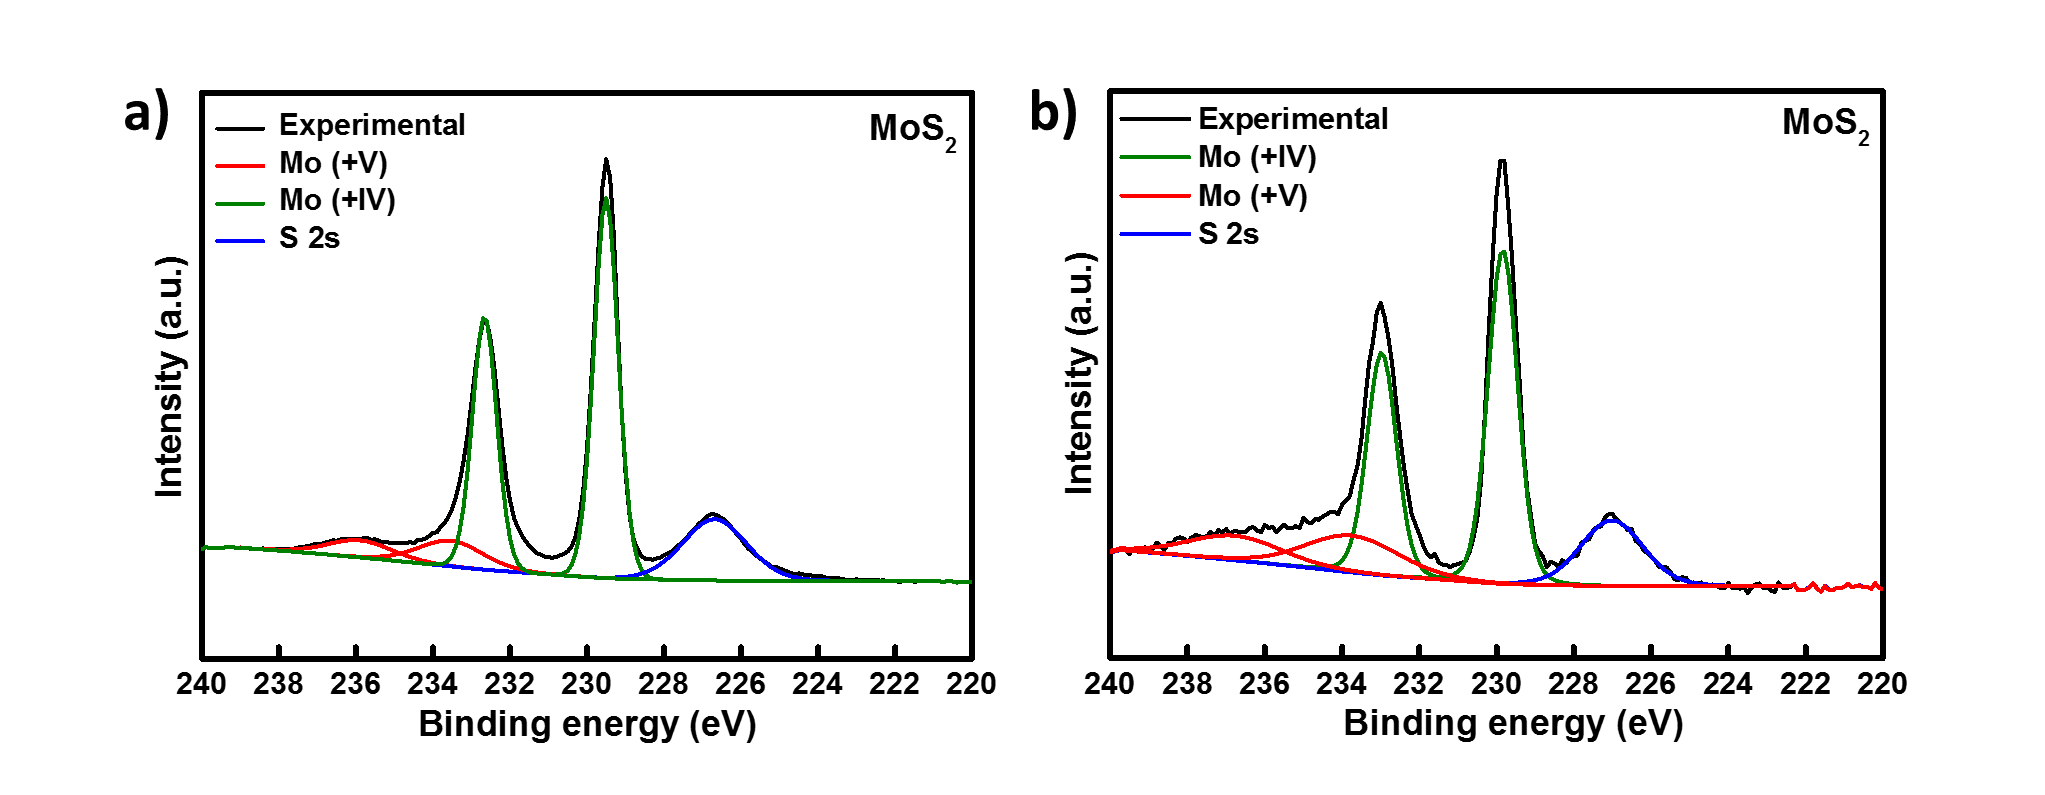
\includegraphics[width=\textwidth]{SF/SF2}
\caption{XPS spectra of Molybdenum 3d for a) pristine and b) charged MoS$_2$ electrodes.\\It was noted that after charge, the quantity of high oxidation state Mo (in red) increased. The chemical environment of Mo atoms change after interaction with chloroaluminates which might be due to formation of an intermediate complex (Al$_x$Cl$_y$.MoS$_2$). The blue peak at 226 eV indicates the 2s peak for Sulfur.}
\end{figure}

\begin{figure}[h!]
\centering
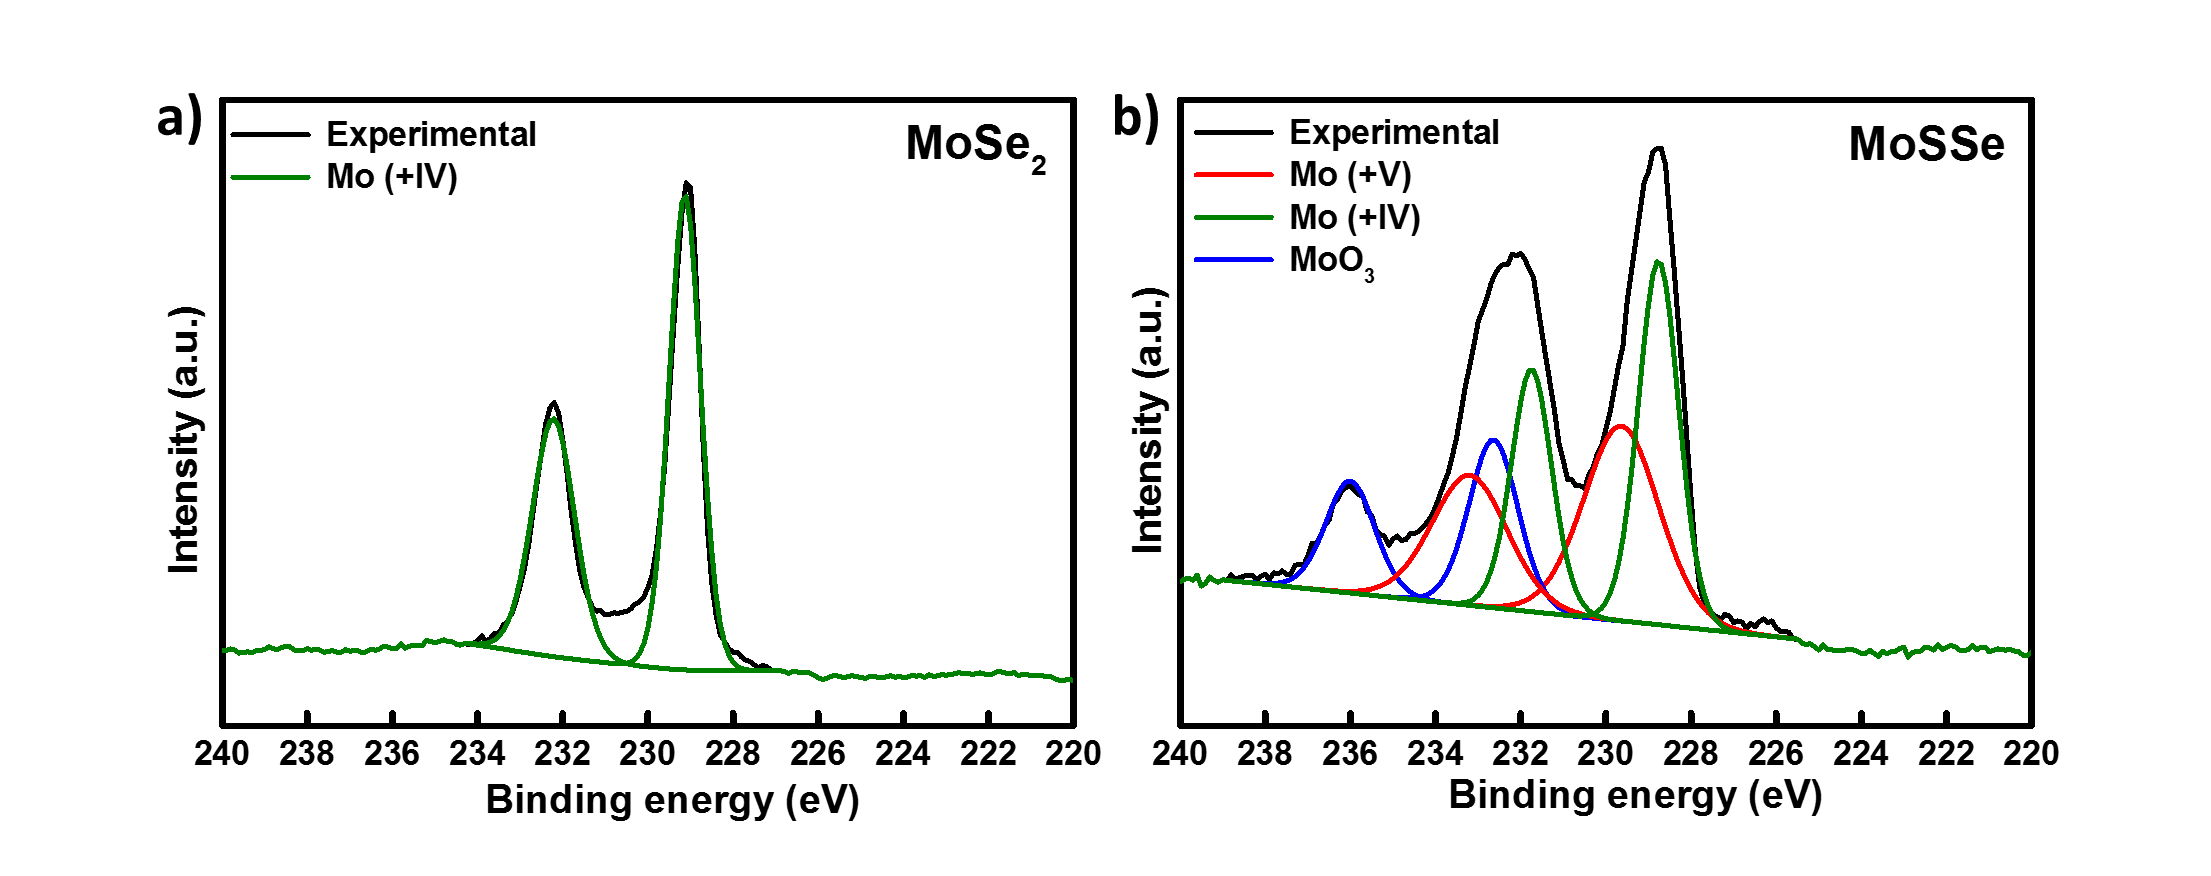
\includegraphics[width=\textwidth]{SF/SF3}
\caption{XPS spectra of Molybdenum 3d for pristine a) MoSe$_2$ and b) MoSSe electrodes.\\For MoSe$_2$, molybdenum observed its pristine peaks at binding energies at 232.2 eV and 229.1 eV depicting Mo$^4^+$ from MoSe$_2$. The Mo peaks in pristine MoSSe electrode observed a complicated spectra. Three doublet peaks appeared corresponding to various oxidation states (Mo$^4^+$ and Mo$^6^+$) with polymorphs 2H and 1T already present. }
\end{figure}

\begin{figure}[h]
\centering
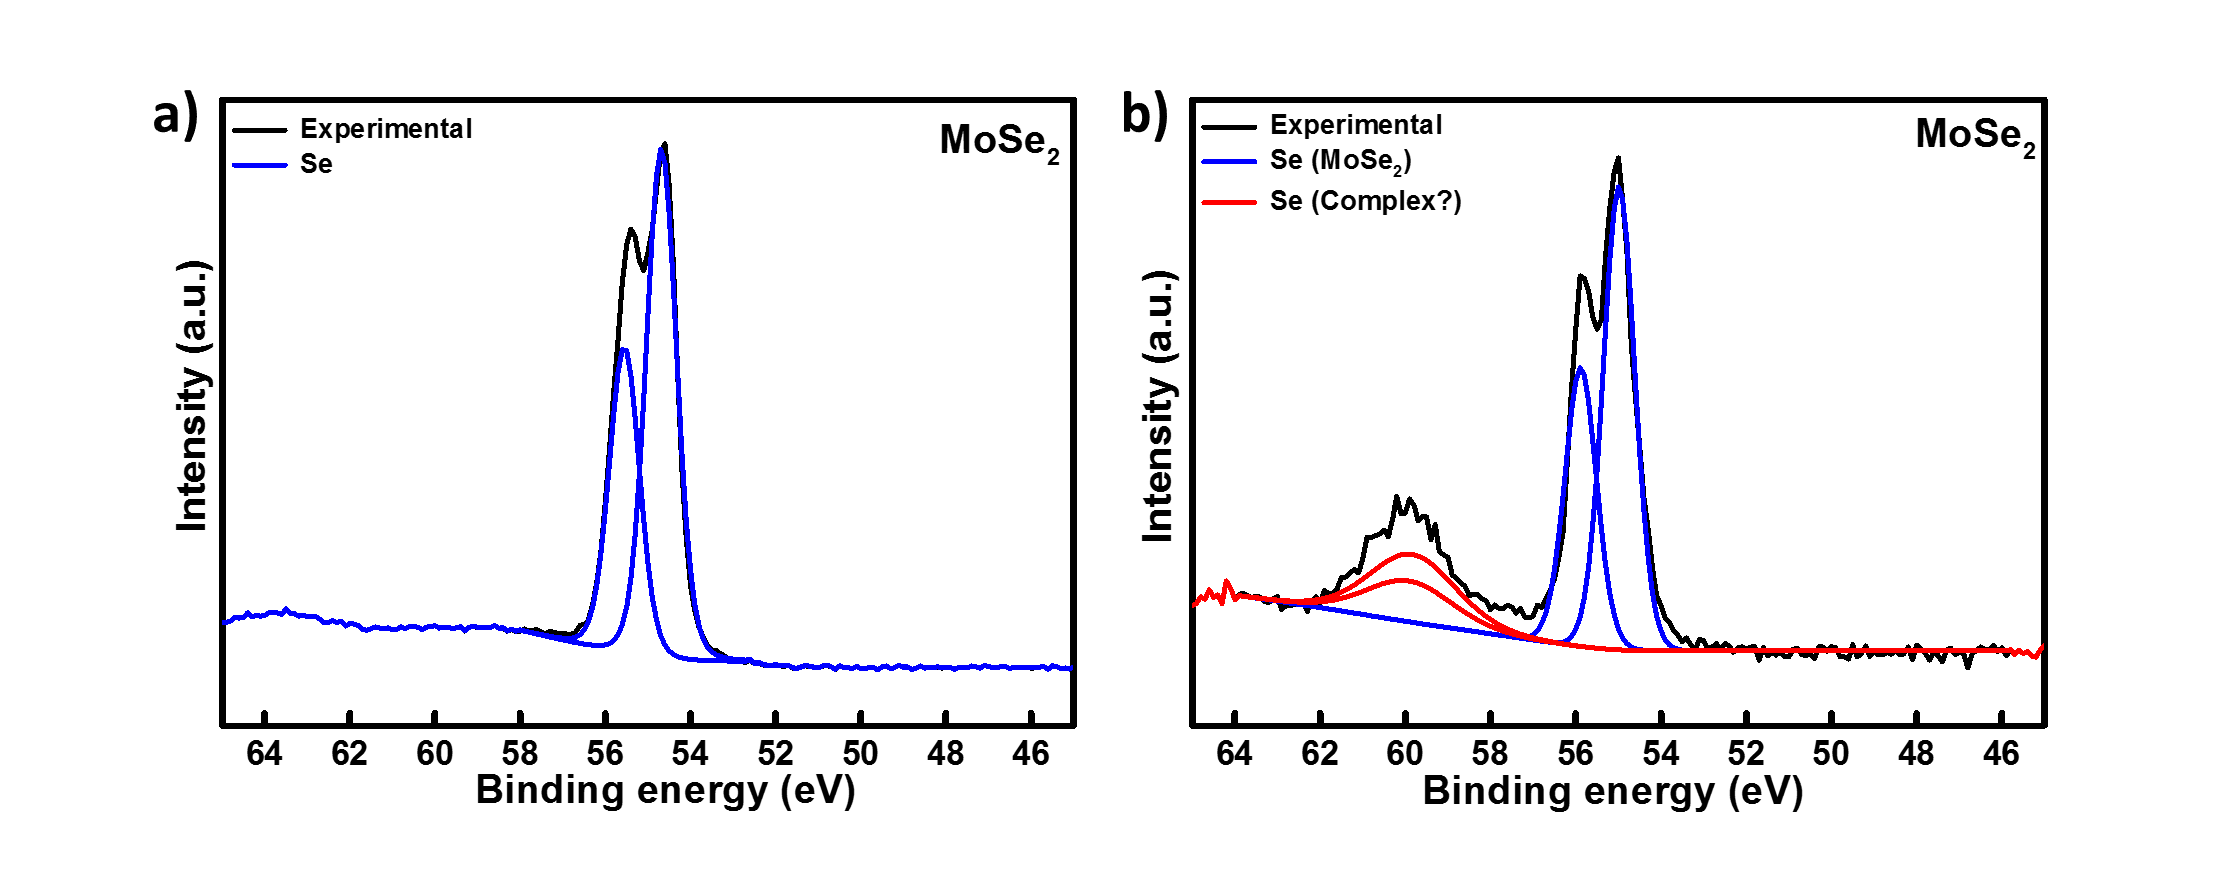
\includegraphics[width=\textwidth]{SF/SF4}
\caption{XPS spectra of Selenium 3d from a) pristine and b) charged electrodes of Al/MoSe$_2$ cell. \\Pristine electrode from MoSe$_2$ observed the characteristic peaks at 55.6 eV and 54.6 eV corresponding to 3d$_3_/_2$ and 3d$_5_/_2$ respectively. After charge, a new peak appeared at 60 eV. We assume this peak arises from a complex (Al$_X$Cl$_y$.MoSe$_2$), which forms when AlCl$_4^-$ intercalate into MoSe$_2$ layers - .}
\end{figure}

\begin{figure}[h]
\centering
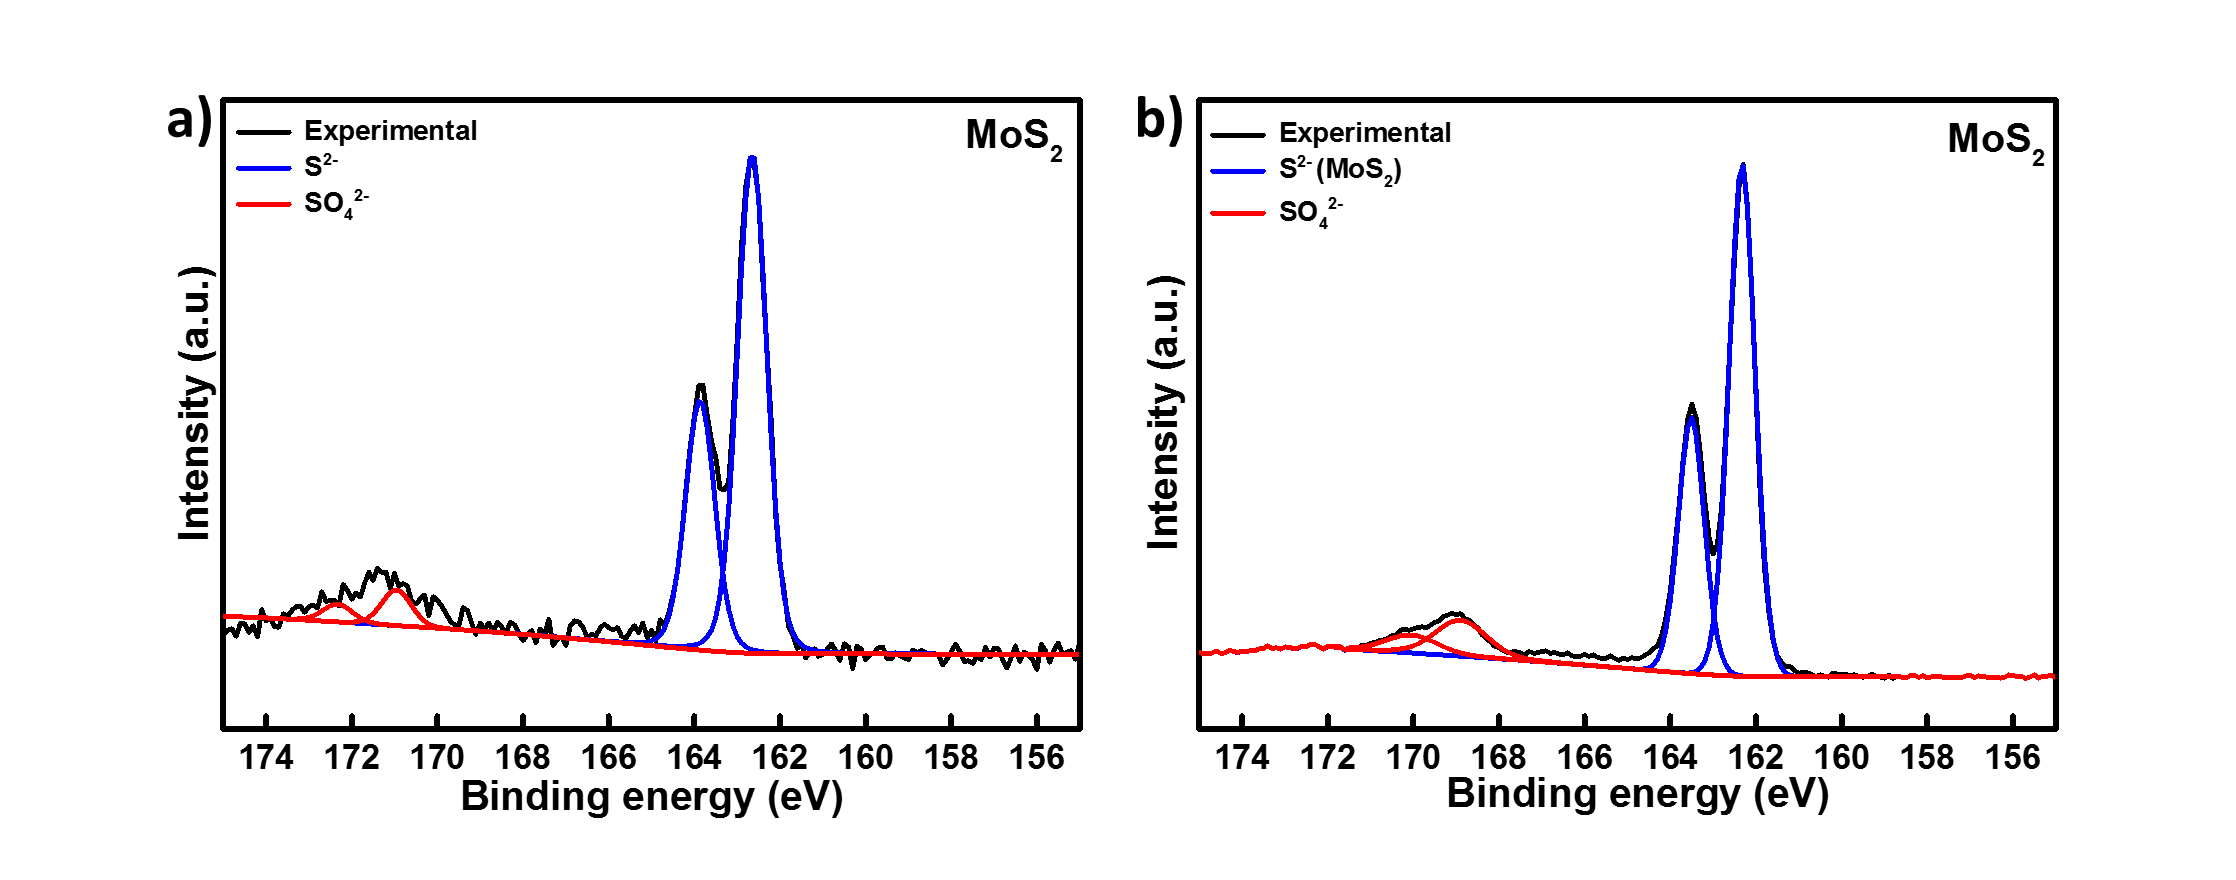
\includegraphics[width=\textwidth]{SF/SF5}
\caption{XPS spectra of Sulfur 2p from a) pristine and b) charged electrodes of Al/MoS$_2$ cell. }
\end{figure}
\begin{figure}[h]
\centering
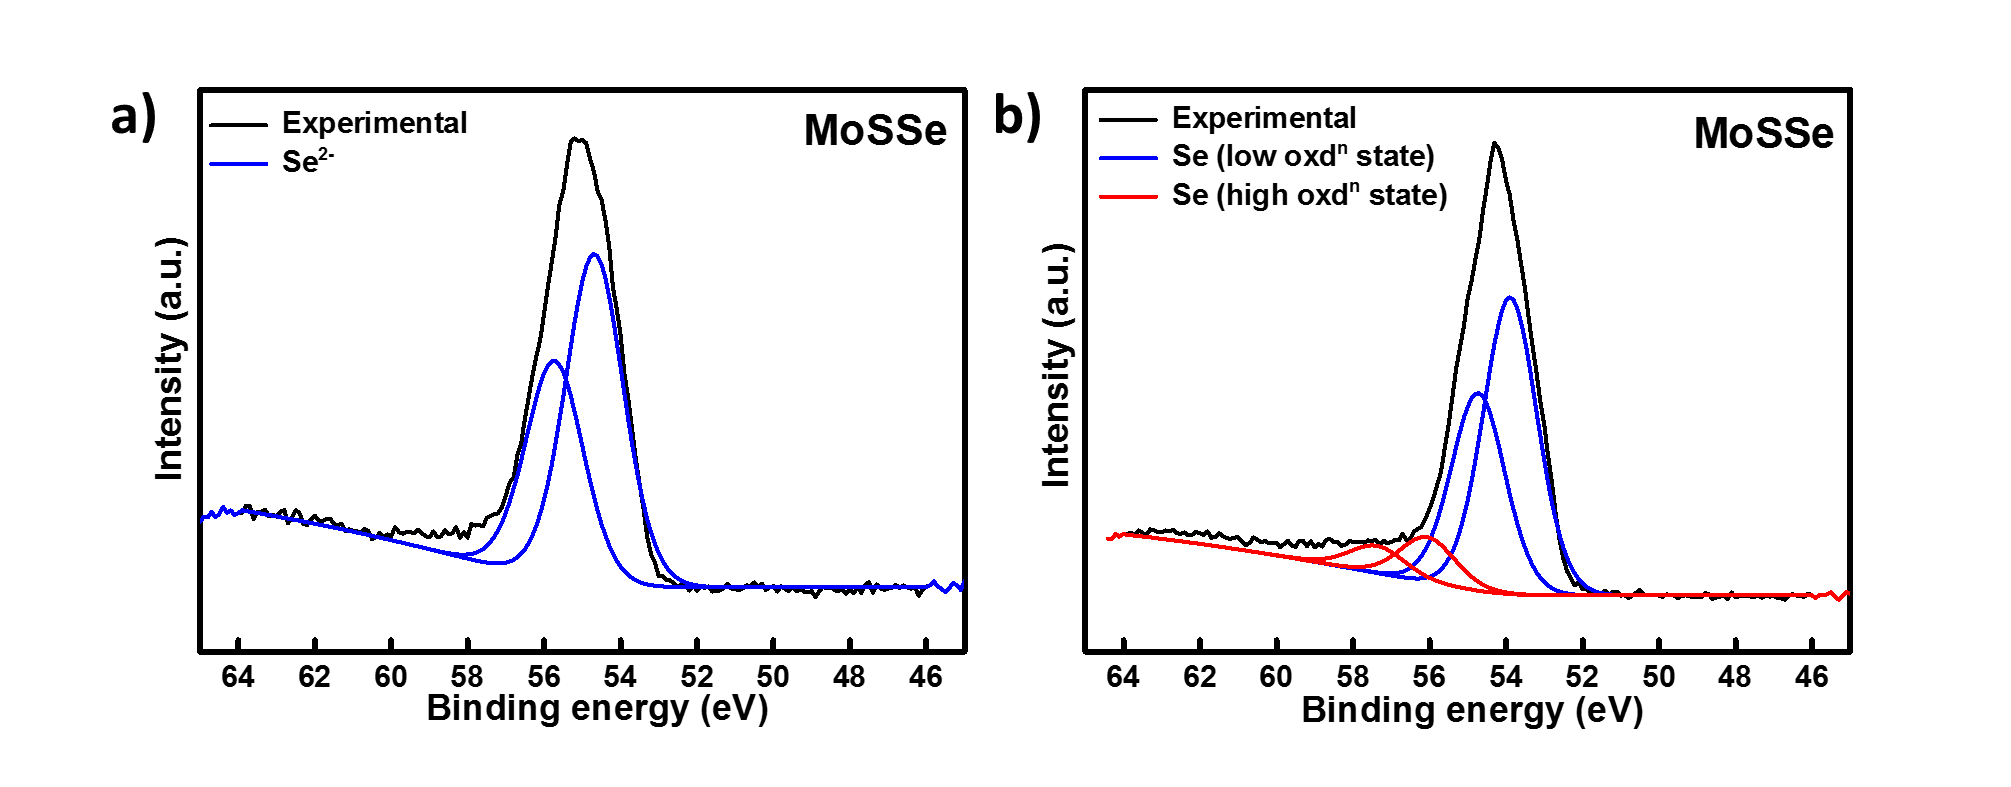
\includegraphics[width=\textwidth]{SF/SF6}
\caption{XPS spectra of Selenium 3d from a) pristine and b) charged electrodes of Al/MoSSe cell.\\Selenium observed a new doublet after charge.}
\end{figure}
\pagebreak



\section*{acknowledgements}
Acknowledgements should include contributions from anyone who does not meet the criteria for authorship (for example, to recognize contributions from people who provided technical help, collation of data, writing assistance, acquisition of funding, or a department chairperson who provided general support), as well as any funding or other support information. 

\section*{Conflict of Interest}
The authors declare no conflict of interest.

\section*{Keywords}
Aluminium-ion battery, molybdenum dichalcogenides, ionic liquid, cathodes


%Bibliography
\bibliography{zoteroBBT_refs}

\pagebreak

\graphicalabstract{figures/ga}{Please check the journal's author guidelines for whether a graphical abstract, key points, new findings, or other items are required for display in the Table of Contents.}


\end{document}


% After this line it is just template stuff - ignore it...
% ----------------------------------------------------------------------

\subsection{Second Level Heading}
If data, scripts or other artefacts used to generate the analyses presented in the article are available via a publicly available data repository, please include a reference to the location of the material within the article.

% Equations should be inserted using standard LaTeX equation and eqnarray environments, not as graphics, and should be set in the main text
This is an equation, numbered
\begin{equation}
\int_0^{+\infty}e^{-x^2}dx=\frac{\sqrt{\pi}}{2}
\end{equation}
And one that is not numbered
\begin{equation*}
e^{i\pi}=-1
\end{equation*}

\subsection{Adding Citations and a References List}

Please use a \verb|.bib| file to store your references. When using Overleaf to prepare your manuscript, you can upload a \verb|.bib| file or import your Mendeley, CiteULike or Zotero library directly as a \verb|.bib| file\footnote{see \url{https://www.overleaf.com/blog/184}}. You can then cite entries from it, like this: \cite{lees2010theoretical}. Just remember to specify a bibliography style, as well as the filename of the \verb|.bib|.

You can find a video tutorial here to learn more about BibTeX: \url{https://www.overleaf.com/help/97-how-to-include-a-bibliography-using-bibtex}.

This template provides two options for the citation and reference list style: 
\begin{description}
\item[Numerical style] Use \verb|\documentclass[...,num-refs]{wiley-article}|
\item[Author-year style] Use \verb|\documentclass[...,alpha-refs]{wiley-article}|
\end{description}

\subsubsection{Third Level Heading}
Supporting information will be included with the published article. For submission any supporting information should be supplied as separate files but referred to in the text.

Appendices will be published after the references. For submission they should be supplied as separate files but referred to in the text.

\paragraph{Fourth Level Heading}
% Here are examples of quotes and epigraphs.
\begin{quote}
The significant problems we have cannot be solved at the same level of thinking with which we created them.\endnote{Albert Einstein said this.}
\end{quote}

\begin{epigraph}{Albert Einstein}
Anyone who has never made a mistake has never tried anything new.
\end{epigraph}

\subparagraph{Fifth level heading}
Measurements should be given in SI or SI-derived units.
Chemical substances should be referred to by the generic name only. Trade names should not be used. Drugs should be referred to by their generic names. If proprietary drugs have been used in the study, refer to these by their generic name, mentioning the proprietary name, and the name and location of the manufacturer, in parentheses.

\begin{table}[bt]
\caption{This is a table. Tables should be self-contained and complement, but not duplicate, information contained in the text. They should be not be provided as images. Legends should be concise but comprehensive – the table, legend and footnotes must be understandable without reference to the text. All abbreviations must be defined in footnotes.}
\begin{threeparttable}
\begin{tabular}{lccrr}
\headrow
\thead{Variables} & \thead{JKL ($\boldsymbol{n=30}$)} & \thead{Control ($\boldsymbol{n=40}$)} & \thead{MN} & \thead{$\boldsymbol t$ (68)}\\
Age at testing & 38 & 58 & 504.48 & 58 ms\\
Age at testing & 38 & 58 & 504.48 & 58 ms\\
Age at testing & 38 & 58 & 504.48 & 58 ms\\
Age at testing & 38 & 58 & 504.48 & 58 ms\\
\hiderowcolors
stop alternating row colors from here onwards\\
Age at testing & 38 & 58 & 504.48 & 58 ms\\
Age at testing & 38 & 58 & 504.48 & 58 ms\\
\hline  % Please only put a hline at the end of the table
\end{tabular}

\begin{tablenotes}
\item JKL, just keep laughing; MN, merry noise.
\end{tablenotes}
\end{threeparttable}
\end{table}

\section*{acknowledgements}
Acknowledgements should include contributions from anyone who does not meet the criteria for authorship (for example, to recognize contributions from people who provided technical help, collation of data, writing assistance, acquisition of funding, or a department chairperson who provided general support), as well as any funding or other support information.

\section*{conflict of interest}
You may be asked to provide a conflict of interest statement during the submission process. Please check the journal's author guidelines for details on what to include in this section. Please ensure you liaise with all co-authors to confirm agreement with the final statement.

\printendnotes

% Submissions are not required to reflect the precise reference formatting of the journal (use of italics, bold etc.), however it is important that all key elements of each reference are included.
\bibliography{sample}

\begin{biography}[example-image-1x1]{A.~One}
Please check with the journal's author guidelines whether author biographies are required. They are usually only included for review-type articles, and typically require photos and brief biographies (up to 75 words) for each author.
\bigskip
\bigskip
\end{biography}

\graphicalabstract{figures/graphical-abstract}{Please check the journal's author guildines for whether a graphical abstract, key points, new findings, or other items are required for display in the Table of Contents.}

%\end{document}
